% Created by tikzDevice version 0.12.3 on 2020-05-26 22:40:36
% !TEX encoding = UTF-8 Unicode
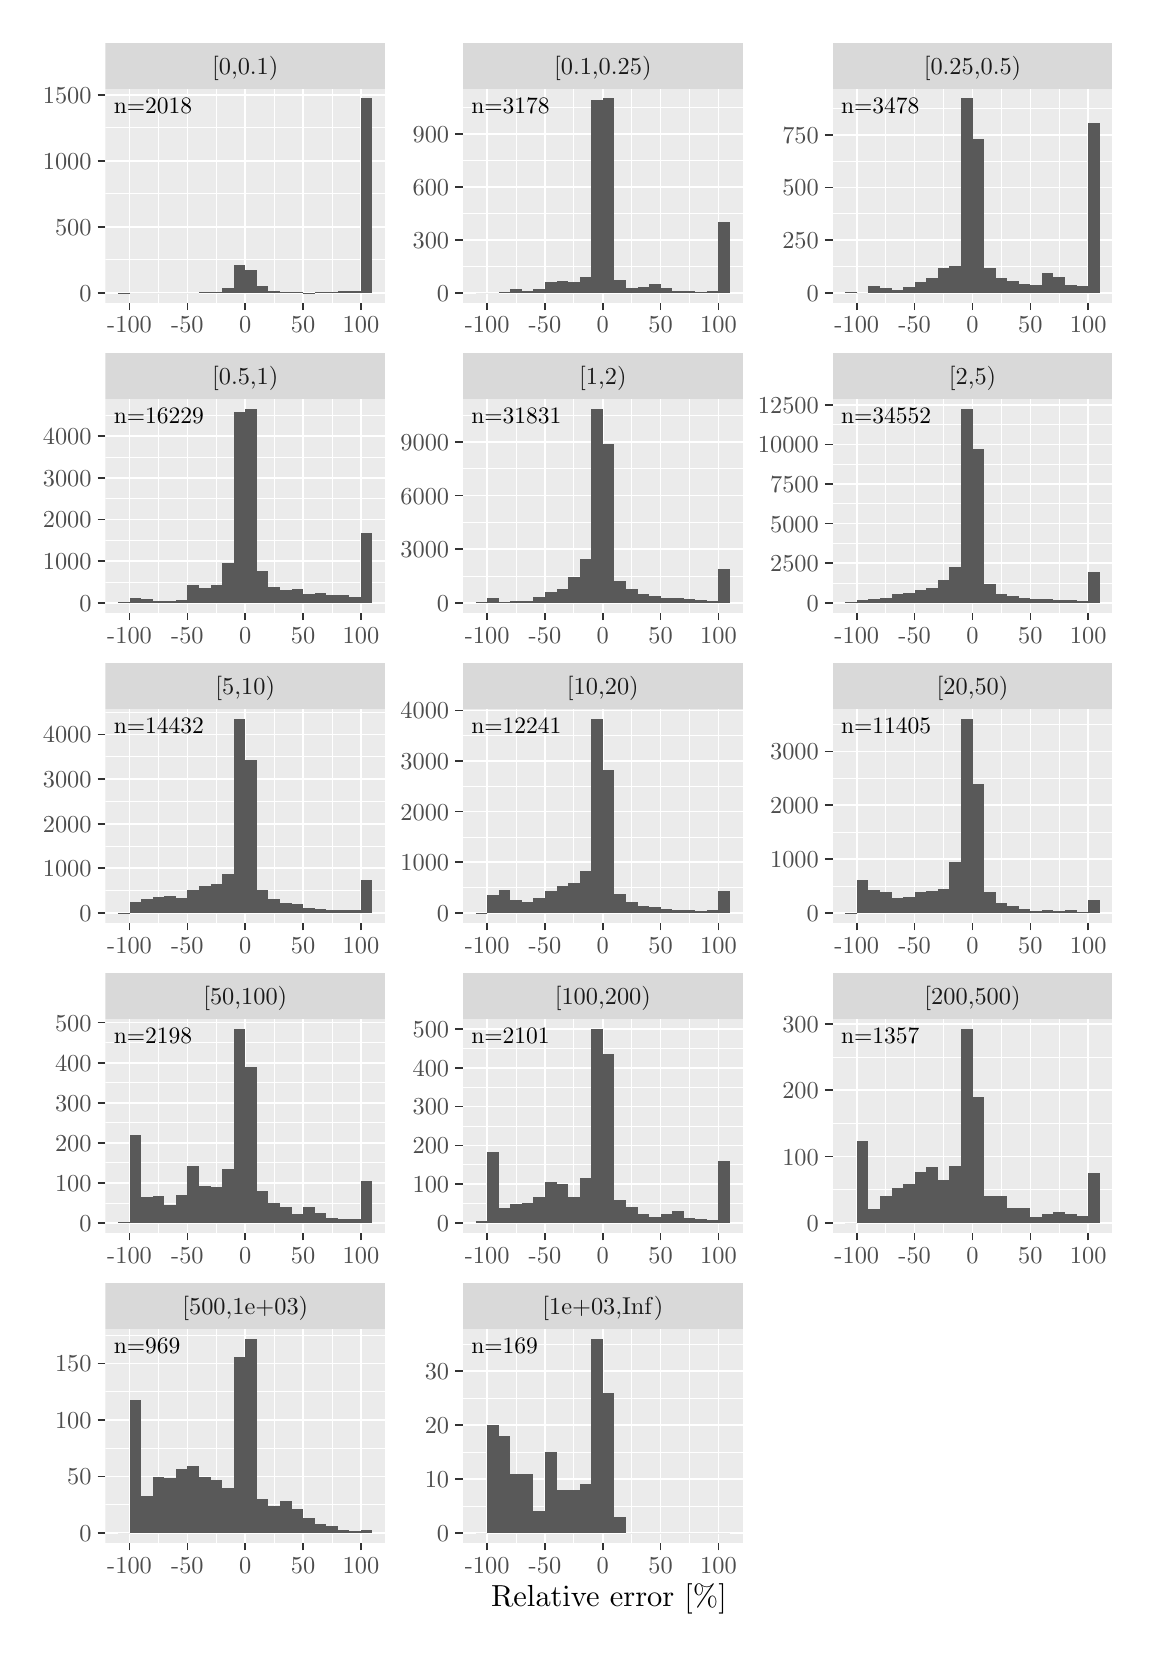
\begin{tikzpicture}[x=1pt,y=1pt]
\definecolor{fillColor}{RGB}{255,255,255}
\path[use as bounding box,fill=fillColor,fill opacity=0.00] (0,0) rectangle (397.48,578.16);
\begin{scope}
\path[clip] (  0.00,  0.00) rectangle (397.48,578.16);
\definecolor{drawColor}{RGB}{255,255,255}
\definecolor{fillColor}{RGB}{255,255,255}

\path[draw=drawColor,line width= 0.6pt,line join=round,line cap=round,fill=fillColor] (  0.00,  0.00) rectangle (397.48,578.16);
\end{scope}
\begin{scope}
\path[clip] ( 28.05,478.84) rectangle (129.20,556.09);
\definecolor{fillColor}{gray}{0.92}

\path[fill=fillColor] ( 28.05,478.84) rectangle (129.20,556.09);
\definecolor{drawColor}{RGB}{255,255,255}

\path[draw=drawColor,line width= 0.3pt,line join=round] ( 28.05,494.27) --
	(129.20,494.27);

\path[draw=drawColor,line width= 0.3pt,line join=round] ( 28.05,518.11) --
	(129.20,518.11);

\path[draw=drawColor,line width= 0.3pt,line join=round] ( 28.05,541.95) --
	(129.20,541.95);

\path[draw=drawColor,line width= 0.3pt,line join=round] ( 47.27,478.84) --
	( 47.27,556.09);

\path[draw=drawColor,line width= 0.3pt,line join=round] ( 68.17,478.84) --
	( 68.17,556.09);

\path[draw=drawColor,line width= 0.3pt,line join=round] ( 89.07,478.84) --
	( 89.07,556.09);

\path[draw=drawColor,line width= 0.3pt,line join=round] (109.97,478.84) --
	(109.97,556.09);

\path[draw=drawColor,line width= 0.6pt,line join=round] ( 28.05,482.35) --
	(129.20,482.35);

\path[draw=drawColor,line width= 0.6pt,line join=round] ( 28.05,506.19) --
	(129.20,506.19);

\path[draw=drawColor,line width= 0.6pt,line join=round] ( 28.05,530.03) --
	(129.20,530.03);

\path[draw=drawColor,line width= 0.6pt,line join=round] ( 28.05,553.86) --
	(129.20,553.86);

\path[draw=drawColor,line width= 0.6pt,line join=round] ( 36.82,478.84) --
	( 36.82,556.09);

\path[draw=drawColor,line width= 0.6pt,line join=round] ( 57.72,478.84) --
	( 57.72,556.09);

\path[draw=drawColor,line width= 0.6pt,line join=round] ( 78.62,478.84) --
	( 78.62,556.09);

\path[draw=drawColor,line width= 0.6pt,line join=round] ( 99.52,478.84) --
	( 99.52,556.09);

\path[draw=drawColor,line width= 0.6pt,line join=round] (120.42,478.84) --
	(120.42,556.09);
\definecolor{fillColor}{gray}{0.35}

\path[fill=fillColor] ( 32.64,482.35) rectangle ( 36.82,482.45);

\path[fill=fillColor] ( 36.82,482.35) rectangle ( 41.00,482.35);

\path[fill=fillColor] ( 41.00,482.35) rectangle ( 45.18,482.35);

\path[fill=fillColor] ( 45.18,482.35) rectangle ( 49.36,482.35);

\path[fill=fillColor] ( 49.36,482.35) rectangle ( 53.54,482.35);

\path[fill=fillColor] ( 53.54,482.35) rectangle ( 57.72,482.35);

\path[fill=fillColor] ( 57.72,482.35) rectangle ( 61.90,482.35);

\path[fill=fillColor] ( 61.90,482.35) rectangle ( 66.08,482.54);

\path[fill=fillColor] ( 66.08,482.35) rectangle ( 70.26,482.64);

\path[fill=fillColor] ( 70.26,482.35) rectangle ( 74.44,484.07);

\path[fill=fillColor] ( 74.44,482.35) rectangle ( 78.62,492.22);

\path[fill=fillColor] ( 78.62,482.35) rectangle ( 82.80,490.65);

\path[fill=fillColor] ( 82.80,482.35) rectangle ( 86.98,484.83);

\path[fill=fillColor] ( 86.98,482.35) rectangle ( 91.16,482.83);

\path[fill=fillColor] ( 91.16,482.35) rectangle ( 95.34,482.69);

\path[fill=fillColor] ( 95.34,482.35) rectangle ( 99.52,482.59);

\path[fill=fillColor] ( 99.52,482.35) rectangle (103.70,482.40);

\path[fill=fillColor] (103.70,482.35) rectangle (107.88,482.64);

\path[fill=fillColor] (107.88,482.35) rectangle (112.06,482.73);

\path[fill=fillColor] (112.06,482.35) rectangle (116.24,482.88);

\path[fill=fillColor] (116.24,482.35) rectangle (120.42,483.12);

\path[fill=fillColor] (120.42,482.35) rectangle (124.60,552.58);
\definecolor{drawColor}{RGB}{0,0,0}

\node[text=drawColor,anchor=base,inner sep=0pt, outer sep=0pt, scale=  0.85] at ( 45.28,547.20) {n=2018};
\end{scope}
\begin{scope}
\path[clip] ( 28.05,366.80) rectangle (129.20,444.05);
\definecolor{fillColor}{gray}{0.92}

\path[fill=fillColor] ( 28.05,366.80) rectangle (129.20,444.05);
\definecolor{drawColor}{RGB}{255,255,255}

\path[draw=drawColor,line width= 0.3pt,line join=round] ( 28.05,377.84) --
	(129.20,377.84);

\path[draw=drawColor,line width= 0.3pt,line join=round] ( 28.05,392.90) --
	(129.20,392.90);

\path[draw=drawColor,line width= 0.3pt,line join=round] ( 28.05,407.96) --
	(129.20,407.96);

\path[draw=drawColor,line width= 0.3pt,line join=round] ( 28.05,423.01) --
	(129.20,423.01);

\path[draw=drawColor,line width= 0.3pt,line join=round] ( 28.05,438.07) --
	(129.20,438.07);

\path[draw=drawColor,line width= 0.3pt,line join=round] ( 47.27,366.80) --
	( 47.27,444.05);

\path[draw=drawColor,line width= 0.3pt,line join=round] ( 68.17,366.80) --
	( 68.17,444.05);

\path[draw=drawColor,line width= 0.3pt,line join=round] ( 89.07,366.80) --
	( 89.07,444.05);

\path[draw=drawColor,line width= 0.3pt,line join=round] (109.97,366.80) --
	(109.97,444.05);

\path[draw=drawColor,line width= 0.6pt,line join=round] ( 28.05,370.31) --
	(129.20,370.31);

\path[draw=drawColor,line width= 0.6pt,line join=round] ( 28.05,385.37) --
	(129.20,385.37);

\path[draw=drawColor,line width= 0.6pt,line join=round] ( 28.05,400.43) --
	(129.20,400.43);

\path[draw=drawColor,line width= 0.6pt,line join=round] ( 28.05,415.48) --
	(129.20,415.48);

\path[draw=drawColor,line width= 0.6pt,line join=round] ( 28.05,430.54) --
	(129.20,430.54);

\path[draw=drawColor,line width= 0.6pt,line join=round] ( 36.82,366.80) --
	( 36.82,444.05);

\path[draw=drawColor,line width= 0.6pt,line join=round] ( 57.72,366.80) --
	( 57.72,444.05);

\path[draw=drawColor,line width= 0.6pt,line join=round] ( 78.62,366.80) --
	( 78.62,444.05);

\path[draw=drawColor,line width= 0.6pt,line join=round] ( 99.52,366.80) --
	( 99.52,444.05);

\path[draw=drawColor,line width= 0.6pt,line join=round] (120.42,366.80) --
	(120.42,444.05);
\definecolor{fillColor}{gray}{0.35}

\path[fill=fillColor] ( 32.64,370.31) rectangle ( 36.82,370.57);

\path[fill=fillColor] ( 36.82,370.31) rectangle ( 41.00,372.21);

\path[fill=fillColor] ( 41.00,370.31) rectangle ( 45.18,371.64);

\path[fill=fillColor] ( 45.18,370.31) rectangle ( 49.36,370.99);

\path[fill=fillColor] ( 49.36,370.31) rectangle ( 53.54,370.93);

\path[fill=fillColor] ( 53.54,370.31) rectangle ( 57.72,371.28);

\path[fill=fillColor] ( 57.72,370.31) rectangle ( 61.90,376.74);

\path[fill=fillColor] ( 61.90,370.31) rectangle ( 66.08,375.67);

\path[fill=fillColor] ( 66.08,370.31) rectangle ( 70.26,376.85);

\path[fill=fillColor] ( 70.26,370.31) rectangle ( 74.44,384.77);

\path[fill=fillColor] ( 74.44,370.31) rectangle ( 78.62,439.23);

\path[fill=fillColor] ( 78.62,370.31) rectangle ( 82.80,440.54);

\path[fill=fillColor] ( 82.80,370.31) rectangle ( 86.98,381.86);

\path[fill=fillColor] ( 86.98,370.31) rectangle ( 91.16,375.98);

\path[fill=fillColor] ( 91.16,370.31) rectangle ( 95.34,375.06);

\path[fill=fillColor] ( 95.34,370.31) rectangle ( 99.52,375.40);

\path[fill=fillColor] ( 99.52,370.31) rectangle (103.70,373.37);

\path[fill=fillColor] (103.70,370.31) rectangle (107.88,373.81);

\path[fill=fillColor] (107.88,370.31) rectangle (112.06,373.25);

\path[fill=fillColor] (112.06,370.31) rectangle (116.24,373.16);

\path[fill=fillColor] (116.24,370.31) rectangle (120.42,372.27);

\path[fill=fillColor] (120.42,370.31) rectangle (124.60,395.68);
\definecolor{drawColor}{RGB}{0,0,0}

\node[text=drawColor,anchor=base,inner sep=0pt, outer sep=0pt, scale=  0.85] at ( 47.41,435.16) {n=16229};
\end{scope}
\begin{scope}
\path[clip] ( 28.05,254.76) rectangle (129.20,332.01);
\definecolor{fillColor}{gray}{0.92}

\path[fill=fillColor] ( 28.05,254.76) rectangle (129.20,332.01);
\definecolor{drawColor}{RGB}{255,255,255}

\path[draw=drawColor,line width= 0.3pt,line join=round] ( 28.05,266.33) --
	(129.20,266.33);

\path[draw=drawColor,line width= 0.3pt,line join=round] ( 28.05,282.44) --
	(129.20,282.44);

\path[draw=drawColor,line width= 0.3pt,line join=round] ( 28.05,298.55) --
	(129.20,298.55);

\path[draw=drawColor,line width= 0.3pt,line join=round] ( 28.05,314.66) --
	(129.20,314.66);

\path[draw=drawColor,line width= 0.3pt,line join=round] ( 28.05,330.77) --
	(129.20,330.77);

\path[draw=drawColor,line width= 0.3pt,line join=round] ( 47.27,254.76) --
	( 47.27,332.01);

\path[draw=drawColor,line width= 0.3pt,line join=round] ( 68.17,254.76) --
	( 68.17,332.01);

\path[draw=drawColor,line width= 0.3pt,line join=round] ( 89.07,254.76) --
	( 89.07,332.01);

\path[draw=drawColor,line width= 0.3pt,line join=round] (109.97,254.76) --
	(109.97,332.01);

\path[draw=drawColor,line width= 0.6pt,line join=round] ( 28.05,258.28) --
	(129.20,258.28);

\path[draw=drawColor,line width= 0.6pt,line join=round] ( 28.05,274.39) --
	(129.20,274.39);

\path[draw=drawColor,line width= 0.6pt,line join=round] ( 28.05,290.50) --
	(129.20,290.50);

\path[draw=drawColor,line width= 0.6pt,line join=round] ( 28.05,306.61) --
	(129.20,306.61);

\path[draw=drawColor,line width= 0.6pt,line join=round] ( 28.05,322.72) --
	(129.20,322.72);

\path[draw=drawColor,line width= 0.6pt,line join=round] ( 36.82,254.76) --
	( 36.82,332.01);

\path[draw=drawColor,line width= 0.6pt,line join=round] ( 57.72,254.76) --
	( 57.72,332.01);

\path[draw=drawColor,line width= 0.6pt,line join=round] ( 78.62,254.76) --
	( 78.62,332.01);

\path[draw=drawColor,line width= 0.6pt,line join=round] ( 99.52,254.76) --
	( 99.52,332.01);

\path[draw=drawColor,line width= 0.6pt,line join=round] (120.42,254.76) --
	(120.42,332.01);
\definecolor{fillColor}{gray}{0.35}

\path[fill=fillColor] ( 32.64,258.28) rectangle ( 36.82,258.42);

\path[fill=fillColor] ( 36.82,258.28) rectangle ( 41.00,262.13);

\path[fill=fillColor] ( 41.00,258.28) rectangle ( 45.18,263.37);

\path[fill=fillColor] ( 45.18,258.28) rectangle ( 49.36,264.06);

\path[fill=fillColor] ( 49.36,258.28) rectangle ( 53.54,264.43);

\path[fill=fillColor] ( 53.54,258.28) rectangle ( 57.72,263.72);

\path[fill=fillColor] ( 57.72,258.28) rectangle ( 61.90,266.59);

\path[fill=fillColor] ( 61.90,258.28) rectangle ( 66.08,268.04);

\path[fill=fillColor] ( 66.08,258.28) rectangle ( 70.26,268.86);

\path[fill=fillColor] ( 70.26,258.28) rectangle ( 74.44,272.36);

\path[fill=fillColor] ( 74.44,258.28) rectangle ( 78.62,328.50);

\path[fill=fillColor] ( 78.62,258.28) rectangle ( 82.80,313.63);

\path[fill=fillColor] ( 82.80,258.28) rectangle ( 86.98,266.49);

\path[fill=fillColor] ( 86.98,258.28) rectangle ( 91.16,263.19);

\path[fill=fillColor] ( 91.16,258.28) rectangle ( 95.34,261.90);

\path[fill=fillColor] ( 95.34,258.28) rectangle ( 99.52,261.38);

\path[fill=fillColor] ( 99.52,258.28) rectangle (103.70,259.97);

\path[fill=fillColor] (103.70,258.28) rectangle (107.88,259.73);

\path[fill=fillColor] (107.88,258.28) rectangle (112.06,259.29);

\path[fill=fillColor] (112.06,258.28) rectangle (116.24,259.16);

\path[fill=fillColor] (116.24,258.28) rectangle (120.42,259.29);

\path[fill=fillColor] (120.42,258.28) rectangle (124.60,270.07);
\definecolor{drawColor}{RGB}{0,0,0}

\node[text=drawColor,anchor=base,inner sep=0pt, outer sep=0pt, scale=  0.85] at ( 47.41,323.12) {n=14432};
\end{scope}
\begin{scope}
\path[clip] ( 28.05,142.72) rectangle (129.20,219.97);
\definecolor{fillColor}{gray}{0.92}

\path[fill=fillColor] ( 28.05,142.72) rectangle (129.20,219.97);
\definecolor{drawColor}{RGB}{255,255,255}

\path[draw=drawColor,line width= 0.3pt,line join=round] ( 28.05,153.48) --
	(129.20,153.48);

\path[draw=drawColor,line width= 0.3pt,line join=round] ( 28.05,167.95) --
	(129.20,167.95);

\path[draw=drawColor,line width= 0.3pt,line join=round] ( 28.05,182.43) --
	(129.20,182.43);

\path[draw=drawColor,line width= 0.3pt,line join=round] ( 28.05,196.91) --
	(129.20,196.91);

\path[draw=drawColor,line width= 0.3pt,line join=round] ( 28.05,211.39) --
	(129.20,211.39);

\path[draw=drawColor,line width= 0.3pt,line join=round] ( 47.27,142.72) --
	( 47.27,219.97);

\path[draw=drawColor,line width= 0.3pt,line join=round] ( 68.17,142.72) --
	( 68.17,219.97);

\path[draw=drawColor,line width= 0.3pt,line join=round] ( 89.07,142.72) --
	( 89.07,219.97);

\path[draw=drawColor,line width= 0.3pt,line join=round] (109.97,142.72) --
	(109.97,219.97);

\path[draw=drawColor,line width= 0.6pt,line join=round] ( 28.05,146.24) --
	(129.20,146.24);

\path[draw=drawColor,line width= 0.6pt,line join=round] ( 28.05,160.72) --
	(129.20,160.72);

\path[draw=drawColor,line width= 0.6pt,line join=round] ( 28.05,175.19) --
	(129.20,175.19);

\path[draw=drawColor,line width= 0.6pt,line join=round] ( 28.05,189.67) --
	(129.20,189.67);

\path[draw=drawColor,line width= 0.6pt,line join=round] ( 28.05,204.15) --
	(129.20,204.15);

\path[draw=drawColor,line width= 0.6pt,line join=round] ( 28.05,218.63) --
	(129.20,218.63);

\path[draw=drawColor,line width= 0.6pt,line join=round] ( 36.82,142.72) --
	( 36.82,219.97);

\path[draw=drawColor,line width= 0.6pt,line join=round] ( 57.72,142.72) --
	( 57.72,219.97);

\path[draw=drawColor,line width= 0.6pt,line join=round] ( 78.62,142.72) --
	( 78.62,219.97);

\path[draw=drawColor,line width= 0.6pt,line join=round] ( 99.52,142.72) --
	( 99.52,219.97);

\path[draw=drawColor,line width= 0.6pt,line join=round] (120.42,142.72) --
	(120.42,219.97);
\definecolor{fillColor}{gray}{0.35}

\path[fill=fillColor] ( 32.64,146.24) rectangle ( 36.82,146.53);

\path[fill=fillColor] ( 36.82,146.24) rectangle ( 41.00,178.09);

\path[fill=fillColor] ( 41.00,146.24) rectangle ( 45.18,155.79);

\path[fill=fillColor] ( 45.18,146.24) rectangle ( 49.36,156.08);

\path[fill=fillColor] ( 49.36,146.24) rectangle ( 53.54,152.61);

\path[fill=fillColor] ( 53.54,146.24) rectangle ( 57.72,156.37);

\path[fill=fillColor] ( 57.72,146.24) rectangle ( 61.90,166.80);

\path[fill=fillColor] ( 61.90,146.24) rectangle ( 66.08,159.56);

\path[fill=fillColor] ( 66.08,146.24) rectangle ( 70.26,159.27);

\path[fill=fillColor] ( 70.26,146.24) rectangle ( 74.44,165.64);

\path[fill=fillColor] ( 74.44,146.24) rectangle ( 78.62,216.46);

\path[fill=fillColor] ( 78.62,146.24) rectangle ( 82.80,202.70);

\path[fill=fillColor] ( 82.80,146.24) rectangle ( 86.98,157.82);

\path[fill=fillColor] ( 86.98,146.24) rectangle ( 91.16,153.62);

\path[fill=fillColor] ( 91.16,146.24) rectangle ( 95.34,151.88);

\path[fill=fillColor] ( 95.34,146.24) rectangle ( 99.52,149.57);

\path[fill=fillColor] ( 99.52,146.24) rectangle (103.70,152.03);

\path[fill=fillColor] (103.70,146.24) rectangle (107.88,149.86);

\path[fill=fillColor] (107.88,146.24) rectangle (112.06,147.97);

\path[fill=fillColor] (112.06,146.24) rectangle (116.24,147.68);

\path[fill=fillColor] (116.24,146.24) rectangle (120.42,147.83);

\path[fill=fillColor] (120.42,146.24) rectangle (124.60,161.29);
\definecolor{drawColor}{RGB}{0,0,0}

\node[text=drawColor,anchor=base,inner sep=0pt, outer sep=0pt, scale=  0.85] at ( 45.28,211.08) {n=2198};
\end{scope}
\begin{scope}
\path[clip] ( 28.05, 30.69) rectangle (129.20,107.93);
\definecolor{fillColor}{gray}{0.92}

\path[fill=fillColor] ( 28.05, 30.69) rectangle (129.20,107.93);
\definecolor{drawColor}{RGB}{255,255,255}

\path[draw=drawColor,line width= 0.3pt,line join=round] ( 28.05, 44.40) --
	(129.20, 44.40);

\path[draw=drawColor,line width= 0.3pt,line join=round] ( 28.05, 64.82) --
	(129.20, 64.82);

\path[draw=drawColor,line width= 0.3pt,line join=round] ( 28.05, 85.23) --
	(129.20, 85.23);

\path[draw=drawColor,line width= 0.3pt,line join=round] ( 28.05,105.65) --
	(129.20,105.65);

\path[draw=drawColor,line width= 0.3pt,line join=round] ( 47.27, 30.69) --
	( 47.27,107.93);

\path[draw=drawColor,line width= 0.3pt,line join=round] ( 68.17, 30.69) --
	( 68.17,107.93);

\path[draw=drawColor,line width= 0.3pt,line join=round] ( 89.07, 30.69) --
	( 89.07,107.93);

\path[draw=drawColor,line width= 0.3pt,line join=round] (109.97, 30.69) --
	(109.97,107.93);

\path[draw=drawColor,line width= 0.6pt,line join=round] ( 28.05, 34.20) --
	(129.20, 34.20);

\path[draw=drawColor,line width= 0.6pt,line join=round] ( 28.05, 54.61) --
	(129.20, 54.61);

\path[draw=drawColor,line width= 0.6pt,line join=round] ( 28.05, 75.02) --
	(129.20, 75.02);

\path[draw=drawColor,line width= 0.6pt,line join=round] ( 28.05, 95.44) --
	(129.20, 95.44);

\path[draw=drawColor,line width= 0.6pt,line join=round] ( 36.82, 30.69) --
	( 36.82,107.93);

\path[draw=drawColor,line width= 0.6pt,line join=round] ( 57.72, 30.69) --
	( 57.72,107.93);

\path[draw=drawColor,line width= 0.6pt,line join=round] ( 78.62, 30.69) --
	( 78.62,107.93);

\path[draw=drawColor,line width= 0.6pt,line join=round] ( 99.52, 30.69) --
	( 99.52,107.93);

\path[draw=drawColor,line width= 0.6pt,line join=round] (120.42, 30.69) --
	(120.42,107.93);
\definecolor{fillColor}{gray}{0.35}

\path[fill=fillColor] ( 32.64, 34.20) rectangle ( 36.82, 34.20);

\path[fill=fillColor] ( 36.82, 34.20) rectangle ( 41.00, 82.37);

\path[fill=fillColor] ( 41.00, 34.20) rectangle ( 45.18, 47.67);

\path[fill=fillColor] ( 45.18, 34.20) rectangle ( 49.36, 54.61);

\path[fill=fillColor] ( 49.36, 34.20) rectangle ( 53.54, 54.20);

\path[fill=fillColor] ( 53.54, 34.20) rectangle ( 57.72, 57.47);

\path[fill=fillColor] ( 57.72, 34.20) rectangle ( 61.90, 58.29);

\path[fill=fillColor] ( 61.90, 34.20) rectangle ( 66.08, 54.61);

\path[fill=fillColor] ( 66.08, 34.20) rectangle ( 70.26, 53.39);

\path[fill=fillColor] ( 70.26, 34.20) rectangle ( 74.44, 50.53);

\path[fill=fillColor] ( 74.44, 34.20) rectangle ( 78.62, 97.89);

\path[fill=fillColor] ( 78.62, 34.20) rectangle ( 82.80,104.42);

\path[fill=fillColor] ( 82.80, 34.20) rectangle ( 86.98, 46.45);

\path[fill=fillColor] ( 86.98, 34.20) rectangle ( 91.16, 44.00);

\path[fill=fillColor] ( 91.16, 34.20) rectangle ( 95.34, 45.63);

\path[fill=fillColor] ( 95.34, 34.20) rectangle ( 99.52, 42.77);

\path[fill=fillColor] ( 99.52, 34.20) rectangle (103.70, 39.50);

\path[fill=fillColor] (103.70, 34.20) rectangle (107.88, 37.46);

\path[fill=fillColor] (107.88, 34.20) rectangle (112.06, 36.65);

\path[fill=fillColor] (112.06, 34.20) rectangle (116.24, 35.42);

\path[fill=fillColor] (116.24, 34.20) rectangle (120.42, 35.01);

\path[fill=fillColor] (120.42, 34.20) rectangle (124.60, 35.42);
\definecolor{drawColor}{RGB}{0,0,0}

\node[text=drawColor,anchor=base,inner sep=0pt, outer sep=0pt, scale=  0.85] at ( 43.15, 99.04) {n=969};
\end{scope}
\begin{scope}
\path[clip] (157.24,478.84) rectangle (258.39,556.09);
\definecolor{fillColor}{gray}{0.92}

\path[fill=fillColor] (157.24,478.84) rectangle (258.39,556.09);
\definecolor{drawColor}{RGB}{255,255,255}

\path[draw=drawColor,line width= 0.3pt,line join=round] (157.24,491.92) --
	(258.39,491.92);

\path[draw=drawColor,line width= 0.3pt,line join=round] (157.24,511.06) --
	(258.39,511.06);

\path[draw=drawColor,line width= 0.3pt,line join=round] (157.24,530.19) --
	(258.39,530.19);

\path[draw=drawColor,line width= 0.3pt,line join=round] (157.24,549.32) --
	(258.39,549.32);

\path[draw=drawColor,line width= 0.3pt,line join=round] (176.47,478.84) --
	(176.47,556.09);

\path[draw=drawColor,line width= 0.3pt,line join=round] (197.37,478.84) --
	(197.37,556.09);

\path[draw=drawColor,line width= 0.3pt,line join=round] (218.27,478.84) --
	(218.27,556.09);

\path[draw=drawColor,line width= 0.3pt,line join=round] (239.16,478.84) --
	(239.16,556.09);

\path[draw=drawColor,line width= 0.6pt,line join=round] (157.24,482.35) --
	(258.39,482.35);

\path[draw=drawColor,line width= 0.6pt,line join=round] (157.24,501.49) --
	(258.39,501.49);

\path[draw=drawColor,line width= 0.6pt,line join=round] (157.24,520.62) --
	(258.39,520.62);

\path[draw=drawColor,line width= 0.6pt,line join=round] (157.24,539.76) --
	(258.39,539.76);

\path[draw=drawColor,line width= 0.6pt,line join=round] (166.02,478.84) --
	(166.02,556.09);

\path[draw=drawColor,line width= 0.6pt,line join=round] (186.92,478.84) --
	(186.92,556.09);

\path[draw=drawColor,line width= 0.6pt,line join=round] (207.82,478.84) --
	(207.82,556.09);

\path[draw=drawColor,line width= 0.6pt,line join=round] (228.71,478.84) --
	(228.71,556.09);

\path[draw=drawColor,line width= 0.6pt,line join=round] (249.61,478.84) --
	(249.61,556.09);
\definecolor{fillColor}{gray}{0.35}

\path[fill=fillColor] (161.84,482.35) rectangle (166.02,482.35);

\path[fill=fillColor] (166.02,482.35) rectangle (170.20,482.35);

\path[fill=fillColor] (170.20,482.35) rectangle (174.38,482.67);

\path[fill=fillColor] (174.38,482.35) rectangle (178.56,483.76);

\path[fill=fillColor] (178.56,482.35) rectangle (182.74,483.12);

\path[fill=fillColor] (182.74,482.35) rectangle (186.92,483.82);

\path[fill=fillColor] (186.92,482.35) rectangle (191.10,486.12);

\path[fill=fillColor] (191.10,482.35) rectangle (195.28,486.63);

\path[fill=fillColor] (195.28,482.35) rectangle (199.46,486.37);

\path[fill=fillColor] (199.46,482.35) rectangle (203.64,488.22);

\path[fill=fillColor] (203.64,482.35) rectangle (207.82,552.07);

\path[fill=fillColor] (207.82,482.35) rectangle (212.00,552.58);

\path[fill=fillColor] (212.00,482.35) rectangle (216.18,486.95);

\path[fill=fillColor] (216.18,482.35) rectangle (220.36,484.01);

\path[fill=fillColor] (220.36,482.35) rectangle (224.53,484.27);

\path[fill=fillColor] (224.53,482.35) rectangle (228.71,485.35);

\path[fill=fillColor] (228.71,482.35) rectangle (232.89,484.08);

\path[fill=fillColor] (232.89,482.35) rectangle (237.07,483.12);

\path[fill=fillColor] (237.07,482.35) rectangle (241.25,482.86);

\path[fill=fillColor] (241.25,482.35) rectangle (245.43,482.80);

\path[fill=fillColor] (245.43,482.35) rectangle (249.61,482.99);

\path[fill=fillColor] (249.61,482.35) rectangle (253.79,507.99);
\definecolor{drawColor}{RGB}{0,0,0}

\node[text=drawColor,anchor=base,inner sep=0pt, outer sep=0pt, scale=  0.85] at (174.48,547.20) {n=3178};
\end{scope}
\begin{scope}
\path[clip] (157.24,366.80) rectangle (258.39,444.05);
\definecolor{fillColor}{gray}{0.92}

\path[fill=fillColor] (157.24,366.80) rectangle (258.39,444.05);
\definecolor{drawColor}{RGB}{255,255,255}

\path[draw=drawColor,line width= 0.3pt,line join=round] (157.24,380.00) --
	(258.39,380.00);

\path[draw=drawColor,line width= 0.3pt,line join=round] (157.24,399.36) --
	(258.39,399.36);

\path[draw=drawColor,line width= 0.3pt,line join=round] (157.24,418.73) --
	(258.39,418.73);

\path[draw=drawColor,line width= 0.3pt,line join=round] (157.24,438.10) --
	(258.39,438.10);

\path[draw=drawColor,line width= 0.3pt,line join=round] (176.47,366.80) --
	(176.47,444.05);

\path[draw=drawColor,line width= 0.3pt,line join=round] (197.37,366.80) --
	(197.37,444.05);

\path[draw=drawColor,line width= 0.3pt,line join=round] (218.27,366.80) --
	(218.27,444.05);

\path[draw=drawColor,line width= 0.3pt,line join=round] (239.16,366.80) --
	(239.16,444.05);

\path[draw=drawColor,line width= 0.6pt,line join=round] (157.24,370.31) --
	(258.39,370.31);

\path[draw=drawColor,line width= 0.6pt,line join=round] (157.24,389.68) --
	(258.39,389.68);

\path[draw=drawColor,line width= 0.6pt,line join=round] (157.24,409.05) --
	(258.39,409.05);

\path[draw=drawColor,line width= 0.6pt,line join=round] (157.24,428.41) --
	(258.39,428.41);

\path[draw=drawColor,line width= 0.6pt,line join=round] (166.02,366.80) --
	(166.02,444.05);

\path[draw=drawColor,line width= 0.6pt,line join=round] (186.92,366.80) --
	(186.92,444.05);

\path[draw=drawColor,line width= 0.6pt,line join=round] (207.82,366.80) --
	(207.82,444.05);

\path[draw=drawColor,line width= 0.6pt,line join=round] (228.71,366.80) --
	(228.71,444.05);

\path[draw=drawColor,line width= 0.6pt,line join=round] (249.61,366.80) --
	(249.61,444.05);
\definecolor{fillColor}{gray}{0.35}

\path[fill=fillColor] (161.84,370.31) rectangle (166.02,370.46);

\path[fill=fillColor] (166.02,370.31) rectangle (170.20,372.08);

\path[fill=fillColor] (170.20,370.31) rectangle (174.38,370.73);

\path[fill=fillColor] (174.38,370.31) rectangle (178.56,370.83);

\path[fill=fillColor] (178.56,370.31) rectangle (182.74,371.11);

\path[fill=fillColor] (182.74,370.31) rectangle (186.92,372.47);

\path[fill=fillColor] (186.92,370.31) rectangle (191.10,374.40);

\path[fill=fillColor] (191.10,370.31) rectangle (195.28,375.44);

\path[fill=fillColor] (195.28,370.31) rectangle (199.46,379.71);

\path[fill=fillColor] (199.46,370.31) rectangle (203.64,386.00);

\path[fill=fillColor] (203.64,370.31) rectangle (207.82,440.54);

\path[fill=fillColor] (207.82,370.31) rectangle (212.00,427.87);

\path[fill=fillColor] (212.00,370.31) rectangle (216.18,378.13);

\path[fill=fillColor] (216.18,370.31) rectangle (220.36,375.30);

\path[fill=fillColor] (220.36,370.31) rectangle (224.53,373.68);

\path[fill=fillColor] (224.53,370.31) rectangle (228.71,372.74);

\path[fill=fillColor] (228.71,370.31) rectangle (232.89,372.19);

\path[fill=fillColor] (232.89,370.31) rectangle (237.07,372.16);

\path[fill=fillColor] (237.07,370.31) rectangle (241.25,371.58);

\path[fill=fillColor] (241.25,370.31) rectangle (245.43,371.32);

\path[fill=fillColor] (245.43,370.31) rectangle (249.61,371.14);

\path[fill=fillColor] (249.61,370.31) rectangle (253.79,382.53);
\definecolor{drawColor}{RGB}{0,0,0}

\node[text=drawColor,anchor=base,inner sep=0pt, outer sep=0pt, scale=  0.85] at (176.61,435.16) {n=31831};
\end{scope}
\begin{scope}
\path[clip] (157.24,254.76) rectangle (258.39,332.01);
\definecolor{fillColor}{gray}{0.92}

\path[fill=fillColor] (157.24,254.76) rectangle (258.39,332.01);
\definecolor{drawColor}{RGB}{255,255,255}

\path[draw=drawColor,line width= 0.3pt,line join=round] (157.24,267.42) --
	(258.39,267.42);

\path[draw=drawColor,line width= 0.3pt,line join=round] (157.24,285.71) --
	(258.39,285.71);

\path[draw=drawColor,line width= 0.3pt,line join=round] (157.24,304.01) --
	(258.39,304.01);

\path[draw=drawColor,line width= 0.3pt,line join=round] (157.24,322.30) --
	(258.39,322.30);

\path[draw=drawColor,line width= 0.3pt,line join=round] (176.47,254.76) --
	(176.47,332.01);

\path[draw=drawColor,line width= 0.3pt,line join=round] (197.37,254.76) --
	(197.37,332.01);

\path[draw=drawColor,line width= 0.3pt,line join=round] (218.27,254.76) --
	(218.27,332.01);

\path[draw=drawColor,line width= 0.3pt,line join=round] (239.16,254.76) --
	(239.16,332.01);

\path[draw=drawColor,line width= 0.6pt,line join=round] (157.24,258.28) --
	(258.39,258.28);

\path[draw=drawColor,line width= 0.6pt,line join=round] (157.24,276.57) --
	(258.39,276.57);

\path[draw=drawColor,line width= 0.6pt,line join=round] (157.24,294.86) --
	(258.39,294.86);

\path[draw=drawColor,line width= 0.6pt,line join=round] (157.24,313.15) --
	(258.39,313.15);

\path[draw=drawColor,line width= 0.6pt,line join=round] (157.24,331.44) --
	(258.39,331.44);

\path[draw=drawColor,line width= 0.6pt,line join=round] (166.02,254.76) --
	(166.02,332.01);

\path[draw=drawColor,line width= 0.6pt,line join=round] (186.92,254.76) --
	(186.92,332.01);

\path[draw=drawColor,line width= 0.6pt,line join=round] (207.82,254.76) --
	(207.82,332.01);

\path[draw=drawColor,line width= 0.6pt,line join=round] (228.71,254.76) --
	(228.71,332.01);

\path[draw=drawColor,line width= 0.6pt,line join=round] (249.61,254.76) --
	(249.61,332.01);
\definecolor{fillColor}{gray}{0.35}

\path[fill=fillColor] (161.84,258.28) rectangle (166.02,258.35);

\path[fill=fillColor] (166.02,258.28) rectangle (170.20,264.70);

\path[fill=fillColor] (170.20,258.28) rectangle (174.38,266.62);

\path[fill=fillColor] (174.38,258.28) rectangle (178.56,262.79);

\path[fill=fillColor] (178.56,258.28) rectangle (182.74,262.21);

\path[fill=fillColor] (182.74,258.28) rectangle (186.92,263.76);

\path[fill=fillColor] (186.92,258.28) rectangle (191.10,266.34);

\path[fill=fillColor] (191.10,258.28) rectangle (195.28,267.97);

\path[fill=fillColor] (195.28,258.28) rectangle (199.46,269.18);

\path[fill=fillColor] (199.46,258.28) rectangle (203.64,273.53);

\path[fill=fillColor] (203.64,258.28) rectangle (207.82,328.50);

\path[fill=fillColor] (207.82,258.28) rectangle (212.00,309.97);

\path[fill=fillColor] (212.00,258.28) rectangle (216.18,265.26);

\path[fill=fillColor] (216.18,258.28) rectangle (220.36,262.24);

\path[fill=fillColor] (220.36,258.28) rectangle (224.53,260.89);

\path[fill=fillColor] (224.53,258.28) rectangle (228.71,260.34);

\path[fill=fillColor] (228.71,258.28) rectangle (232.89,259.57);

\path[fill=fillColor] (232.89,258.28) rectangle (237.07,259.46);

\path[fill=fillColor] (237.07,258.28) rectangle (241.25,259.39);

\path[fill=fillColor] (241.25,258.28) rectangle (245.43,259.14);

\path[fill=fillColor] (245.43,258.28) rectangle (249.61,259.43);

\path[fill=fillColor] (249.61,258.28) rectangle (253.79,266.32);
\definecolor{drawColor}{RGB}{0,0,0}

\node[text=drawColor,anchor=base,inner sep=0pt, outer sep=0pt, scale=  0.85] at (176.61,323.12) {n=12241};
\end{scope}
\begin{scope}
\path[clip] (157.24,142.72) rectangle (258.39,219.97);
\definecolor{fillColor}{gray}{0.92}

\path[fill=fillColor] (157.24,142.72) rectangle (258.39,219.97);
\definecolor{drawColor}{RGB}{255,255,255}

\path[draw=drawColor,line width= 0.3pt,line join=round] (157.24,153.24) --
	(258.39,153.24);

\path[draw=drawColor,line width= 0.3pt,line join=round] (157.24,167.26) --
	(258.39,167.26);

\path[draw=drawColor,line width= 0.3pt,line join=round] (157.24,181.28) --
	(258.39,181.28);

\path[draw=drawColor,line width= 0.3pt,line join=round] (157.24,195.29) --
	(258.39,195.29);

\path[draw=drawColor,line width= 0.3pt,line join=round] (157.24,209.31) --
	(258.39,209.31);

\path[draw=drawColor,line width= 0.3pt,line join=round] (176.47,142.72) --
	(176.47,219.97);

\path[draw=drawColor,line width= 0.3pt,line join=round] (197.37,142.72) --
	(197.37,219.97);

\path[draw=drawColor,line width= 0.3pt,line join=round] (218.27,142.72) --
	(218.27,219.97);

\path[draw=drawColor,line width= 0.3pt,line join=round] (239.16,142.72) --
	(239.16,219.97);

\path[draw=drawColor,line width= 0.6pt,line join=round] (157.24,146.24) --
	(258.39,146.24);

\path[draw=drawColor,line width= 0.6pt,line join=round] (157.24,160.25) --
	(258.39,160.25);

\path[draw=drawColor,line width= 0.6pt,line join=round] (157.24,174.27) --
	(258.39,174.27);

\path[draw=drawColor,line width= 0.6pt,line join=round] (157.24,188.29) --
	(258.39,188.29);

\path[draw=drawColor,line width= 0.6pt,line join=round] (157.24,202.30) --
	(258.39,202.30);

\path[draw=drawColor,line width= 0.6pt,line join=round] (157.24,216.32) --
	(258.39,216.32);

\path[draw=drawColor,line width= 0.6pt,line join=round] (166.02,142.72) --
	(166.02,219.97);

\path[draw=drawColor,line width= 0.6pt,line join=round] (186.92,142.72) --
	(186.92,219.97);

\path[draw=drawColor,line width= 0.6pt,line join=round] (207.82,142.72) --
	(207.82,219.97);

\path[draw=drawColor,line width= 0.6pt,line join=round] (228.71,142.72) --
	(228.71,219.97);

\path[draw=drawColor,line width= 0.6pt,line join=round] (249.61,142.72) --
	(249.61,219.97);
\definecolor{fillColor}{gray}{0.35}

\path[fill=fillColor] (161.84,146.24) rectangle (166.02,146.80);

\path[fill=fillColor] (166.02,146.24) rectangle (170.20,172.03);

\path[fill=fillColor] (170.20,146.24) rectangle (174.38,151.56);

\path[fill=fillColor] (174.38,146.24) rectangle (178.56,152.96);

\path[fill=fillColor] (178.56,146.24) rectangle (182.74,153.52);

\path[fill=fillColor] (182.74,146.24) rectangle (186.92,155.77);

\path[fill=fillColor] (186.92,146.24) rectangle (191.10,161.09);

\path[fill=fillColor] (191.10,146.24) rectangle (195.28,160.25);

\path[fill=fillColor] (195.28,146.24) rectangle (199.46,155.63);

\path[fill=fillColor] (199.46,146.24) rectangle (203.64,162.36);

\path[fill=fillColor] (203.64,146.24) rectangle (207.82,216.46);

\path[fill=fillColor] (207.82,146.24) rectangle (212.00,207.21);

\path[fill=fillColor] (212.00,146.24) rectangle (216.18,154.37);

\path[fill=fillColor] (216.18,146.24) rectangle (220.36,151.98);

\path[fill=fillColor] (220.36,146.24) rectangle (224.53,149.32);

\path[fill=fillColor] (224.53,146.24) rectangle (228.71,148.34);

\path[fill=fillColor] (228.71,146.24) rectangle (232.89,149.60);

\path[fill=fillColor] (232.89,146.24) rectangle (237.07,150.72);

\path[fill=fillColor] (237.07,146.24) rectangle (241.25,147.92);

\path[fill=fillColor] (241.25,146.24) rectangle (245.43,147.78);

\path[fill=fillColor] (245.43,146.24) rectangle (249.61,147.36);

\path[fill=fillColor] (249.61,146.24) rectangle (253.79,168.66);
\definecolor{drawColor}{RGB}{0,0,0}

\node[text=drawColor,anchor=base,inner sep=0pt, outer sep=0pt, scale=  0.85] at (174.48,211.08) {n=2101};
\end{scope}
\begin{scope}
\path[clip] (157.24, 30.69) rectangle (258.39,107.93);
\definecolor{fillColor}{gray}{0.92}

\path[fill=fillColor] (157.24, 30.69) rectangle (258.39,107.93);
\definecolor{drawColor}{RGB}{255,255,255}

\path[draw=drawColor,line width= 0.3pt,line join=round] (157.24, 43.95) --
	(258.39, 43.95);

\path[draw=drawColor,line width= 0.3pt,line join=round] (157.24, 63.46) --
	(258.39, 63.46);

\path[draw=drawColor,line width= 0.3pt,line join=round] (157.24, 82.96) --
	(258.39, 82.96);

\path[draw=drawColor,line width= 0.3pt,line join=round] (157.24,102.47) --
	(258.39,102.47);

\path[draw=drawColor,line width= 0.3pt,line join=round] (176.47, 30.69) --
	(176.47,107.93);

\path[draw=drawColor,line width= 0.3pt,line join=round] (197.37, 30.69) --
	(197.37,107.93);

\path[draw=drawColor,line width= 0.3pt,line join=round] (218.27, 30.69) --
	(218.27,107.93);

\path[draw=drawColor,line width= 0.3pt,line join=round] (239.16, 30.69) --
	(239.16,107.93);

\path[draw=drawColor,line width= 0.6pt,line join=round] (157.24, 34.20) --
	(258.39, 34.20);

\path[draw=drawColor,line width= 0.6pt,line join=round] (157.24, 53.70) --
	(258.39, 53.70);

\path[draw=drawColor,line width= 0.6pt,line join=round] (157.24, 73.21) --
	(258.39, 73.21);

\path[draw=drawColor,line width= 0.6pt,line join=round] (157.24, 92.72) --
	(258.39, 92.72);

\path[draw=drawColor,line width= 0.6pt,line join=round] (166.02, 30.69) --
	(166.02,107.93);

\path[draw=drawColor,line width= 0.6pt,line join=round] (186.92, 30.69) --
	(186.92,107.93);

\path[draw=drawColor,line width= 0.6pt,line join=round] (207.82, 30.69) --
	(207.82,107.93);

\path[draw=drawColor,line width= 0.6pt,line join=round] (228.71, 30.69) --
	(228.71,107.93);

\path[draw=drawColor,line width= 0.6pt,line join=round] (249.61, 30.69) --
	(249.61,107.93);
\definecolor{fillColor}{gray}{0.35}

\path[fill=fillColor] (161.84, 34.20) rectangle (166.02, 34.20);

\path[fill=fillColor] (166.02, 34.20) rectangle (170.20, 73.21);

\path[fill=fillColor] (170.20, 34.20) rectangle (174.38, 69.31);

\path[fill=fillColor] (174.38, 34.20) rectangle (178.56, 55.65);

\path[fill=fillColor] (178.56, 34.20) rectangle (182.74, 55.65);

\path[fill=fillColor] (182.74, 34.20) rectangle (186.92, 42.00);

\path[fill=fillColor] (186.92, 34.20) rectangle (191.10, 63.46);

\path[fill=fillColor] (191.10, 34.20) rectangle (195.28, 49.80);

\path[fill=fillColor] (195.28, 34.20) rectangle (199.46, 49.80);

\path[fill=fillColor] (199.46, 34.20) rectangle (203.64, 51.75);

\path[fill=fillColor] (203.64, 34.20) rectangle (207.82,104.42);

\path[fill=fillColor] (207.82, 34.20) rectangle (212.00, 84.91);

\path[fill=fillColor] (212.00, 34.20) rectangle (216.18, 40.05);

\path[fill=fillColor] (216.18, 34.20) rectangle (220.36, 34.20);

\path[fill=fillColor] (220.36, 34.20) rectangle (224.53, 34.20);

\path[fill=fillColor] (224.53, 34.20) rectangle (228.71, 34.20);

\path[fill=fillColor] (228.71, 34.20) rectangle (232.89, 34.20);

\path[fill=fillColor] (232.89, 34.20) rectangle (237.07, 34.20);

\path[fill=fillColor] (237.07, 34.20) rectangle (241.25, 34.20);

\path[fill=fillColor] (241.25, 34.20) rectangle (245.43, 34.20);

\path[fill=fillColor] (245.43, 34.20) rectangle (249.61, 34.20);

\path[fill=fillColor] (249.61, 34.20) rectangle (253.79, 34.20);
\definecolor{drawColor}{RGB}{0,0,0}

\node[text=drawColor,anchor=base,inner sep=0pt, outer sep=0pt, scale=  0.85] at (172.34, 99.04) {n=169};
\end{scope}
\begin{scope}
\path[clip] (290.84,478.84) rectangle (391.98,556.09);
\definecolor{fillColor}{gray}{0.92}

\path[fill=fillColor] (290.84,478.84) rectangle (391.98,556.09);
\definecolor{drawColor}{RGB}{255,255,255}

\path[draw=drawColor,line width= 0.3pt,line join=round] (290.84,491.87) --
	(391.98,491.87);

\path[draw=drawColor,line width= 0.3pt,line join=round] (290.84,510.92) --
	(391.98,510.92);

\path[draw=drawColor,line width= 0.3pt,line join=round] (290.84,529.96) --
	(391.98,529.96);

\path[draw=drawColor,line width= 0.3pt,line join=round] (290.84,549.00) --
	(391.98,549.00);

\path[draw=drawColor,line width= 0.3pt,line join=round] (310.06,478.84) --
	(310.06,556.09);

\path[draw=drawColor,line width= 0.3pt,line join=round] (330.96,478.84) --
	(330.96,556.09);

\path[draw=drawColor,line width= 0.3pt,line join=round] (351.86,478.84) --
	(351.86,556.09);

\path[draw=drawColor,line width= 0.3pt,line join=round] (372.76,478.84) --
	(372.76,556.09);

\path[draw=drawColor,line width= 0.6pt,line join=round] (290.84,482.35) --
	(391.98,482.35);

\path[draw=drawColor,line width= 0.6pt,line join=round] (290.84,501.39) --
	(391.98,501.39);

\path[draw=drawColor,line width= 0.6pt,line join=round] (290.84,520.44) --
	(391.98,520.44);

\path[draw=drawColor,line width= 0.6pt,line join=round] (290.84,539.48) --
	(391.98,539.48);

\path[draw=drawColor,line width= 0.6pt,line join=round] (299.61,478.84) --
	(299.61,556.09);

\path[draw=drawColor,line width= 0.6pt,line join=round] (320.51,478.84) --
	(320.51,556.09);

\path[draw=drawColor,line width= 0.6pt,line join=round] (341.41,478.84) --
	(341.41,556.09);

\path[draw=drawColor,line width= 0.6pt,line join=round] (362.31,478.84) --
	(362.31,556.09);

\path[draw=drawColor,line width= 0.6pt,line join=round] (383.21,478.84) --
	(383.21,556.09);
\definecolor{fillColor}{gray}{0.35}

\path[fill=fillColor] (295.43,482.35) rectangle (299.61,482.58);

\path[fill=fillColor] (299.61,482.35) rectangle (303.79,482.35);

\path[fill=fillColor] (303.79,482.35) rectangle (307.97,484.94);

\path[fill=fillColor] (307.97,482.35) rectangle (312.15,484.11);

\path[fill=fillColor] (312.15,482.35) rectangle (316.33,483.19);

\path[fill=fillColor] (316.33,482.35) rectangle (320.51,484.41);

\path[fill=fillColor] (320.51,482.35) rectangle (324.69,486.16);

\path[fill=fillColor] (324.69,482.35) rectangle (328.87,487.53);

\path[fill=fillColor] (328.87,482.35) rectangle (333.05,491.49);

\path[fill=fillColor] (333.05,482.35) rectangle (337.23,492.03);

\path[fill=fillColor] (337.23,482.35) rectangle (341.41,552.58);

\path[fill=fillColor] (341.41,482.35) rectangle (345.59,537.88);

\path[fill=fillColor] (345.59,482.35) rectangle (349.77,491.26);

\path[fill=fillColor] (349.77,482.35) rectangle (353.95,487.61);

\path[fill=fillColor] (353.95,482.35) rectangle (358.13,486.62);

\path[fill=fillColor] (358.13,482.35) rectangle (362.31,485.70);

\path[fill=fillColor] (362.31,482.35) rectangle (366.49,485.17);

\path[fill=fillColor] (366.49,482.35) rectangle (370.67,489.36);

\path[fill=fillColor] (370.67,482.35) rectangle (374.85,487.99);

\path[fill=fillColor] (374.85,482.35) rectangle (379.03,485.25);

\path[fill=fillColor] (379.03,482.35) rectangle (383.21,484.71);

\path[fill=fillColor] (383.21,482.35) rectangle (387.39,543.74);
\definecolor{drawColor}{RGB}{0,0,0}

\node[text=drawColor,anchor=base,inner sep=0pt, outer sep=0pt, scale=  0.85] at (308.07,547.20) {n=3478};
\end{scope}
\begin{scope}
\path[clip] (290.84,366.80) rectangle (391.98,444.05);
\definecolor{fillColor}{gray}{0.92}

\path[fill=fillColor] (290.84,366.80) rectangle (391.98,444.05);
\definecolor{drawColor}{RGB}{255,255,255}

\path[draw=drawColor,line width= 0.3pt,line join=round] (290.84,377.47) --
	(391.98,377.47);

\path[draw=drawColor,line width= 0.3pt,line join=round] (290.84,391.79) --
	(391.98,391.79);

\path[draw=drawColor,line width= 0.3pt,line join=round] (290.84,406.11) --
	(391.98,406.11);

\path[draw=drawColor,line width= 0.3pt,line join=round] (290.84,420.43) --
	(391.98,420.43);

\path[draw=drawColor,line width= 0.3pt,line join=round] (290.84,434.75) --
	(391.98,434.75);

\path[draw=drawColor,line width= 0.3pt,line join=round] (310.06,366.80) --
	(310.06,444.05);

\path[draw=drawColor,line width= 0.3pt,line join=round] (330.96,366.80) --
	(330.96,444.05);

\path[draw=drawColor,line width= 0.3pt,line join=round] (351.86,366.80) --
	(351.86,444.05);

\path[draw=drawColor,line width= 0.3pt,line join=round] (372.76,366.80) --
	(372.76,444.05);

\path[draw=drawColor,line width= 0.6pt,line join=round] (290.84,370.31) --
	(391.98,370.31);

\path[draw=drawColor,line width= 0.6pt,line join=round] (290.84,384.63) --
	(391.98,384.63);

\path[draw=drawColor,line width= 0.6pt,line join=round] (290.84,398.95) --
	(391.98,398.95);

\path[draw=drawColor,line width= 0.6pt,line join=round] (290.84,413.27) --
	(391.98,413.27);

\path[draw=drawColor,line width= 0.6pt,line join=round] (290.84,427.59) --
	(391.98,427.59);

\path[draw=drawColor,line width= 0.6pt,line join=round] (290.84,441.91) --
	(391.98,441.91);

\path[draw=drawColor,line width= 0.6pt,line join=round] (299.61,366.80) --
	(299.61,444.05);

\path[draw=drawColor,line width= 0.6pt,line join=round] (320.51,366.80) --
	(320.51,444.05);

\path[draw=drawColor,line width= 0.6pt,line join=round] (341.41,366.80) --
	(341.41,444.05);

\path[draw=drawColor,line width= 0.6pt,line join=round] (362.31,366.80) --
	(362.31,444.05);

\path[draw=drawColor,line width= 0.6pt,line join=round] (383.21,366.80) --
	(383.21,444.05);
\definecolor{fillColor}{gray}{0.35}

\path[fill=fillColor] (295.43,370.31) rectangle (299.61,370.54);

\path[fill=fillColor] (299.61,370.31) rectangle (303.79,371.28);

\path[fill=fillColor] (303.79,370.31) rectangle (307.97,371.61);

\path[fill=fillColor] (307.97,370.31) rectangle (312.15,372.11);

\path[fill=fillColor] (312.15,370.31) rectangle (316.33,373.36);

\path[fill=fillColor] (316.33,370.31) rectangle (320.51,373.91);

\path[fill=fillColor] (320.51,370.31) rectangle (324.69,374.90);

\path[fill=fillColor] (324.69,370.31) rectangle (328.87,375.69);

\path[fill=fillColor] (328.87,370.31) rectangle (333.05,378.59);

\path[fill=fillColor] (333.05,370.31) rectangle (337.23,383.13);

\path[fill=fillColor] (337.23,370.31) rectangle (341.41,440.54);

\path[fill=fillColor] (341.41,370.31) rectangle (345.59,425.82);

\path[fill=fillColor] (345.59,370.31) rectangle (349.77,377.04);

\path[fill=fillColor] (349.77,370.31) rectangle (353.95,373.52);

\path[fill=fillColor] (353.95,370.31) rectangle (358.13,372.89);

\path[fill=fillColor] (358.13,370.31) rectangle (362.31,372.00);

\path[fill=fillColor] (362.31,370.31) rectangle (366.49,371.73);

\path[fill=fillColor] (366.49,370.31) rectangle (370.67,371.59);

\path[fill=fillColor] (370.67,370.31) rectangle (374.85,371.18);

\path[fill=fillColor] (374.85,370.31) rectangle (379.03,371.18);

\path[fill=fillColor] (379.03,370.31) rectangle (383.21,370.92);

\path[fill=fillColor] (383.21,370.31) rectangle (387.39,381.29);
\definecolor{drawColor}{RGB}{0,0,0}

\node[text=drawColor,anchor=base,inner sep=0pt, outer sep=0pt, scale=  0.85] at (310.20,435.16) {n=34552};
\end{scope}
\begin{scope}
\path[clip] (290.84,254.76) rectangle (391.98,332.01);
\definecolor{fillColor}{gray}{0.92}

\path[fill=fillColor] (290.84,254.76) rectangle (391.98,332.01);
\definecolor{drawColor}{RGB}{255,255,255}

\path[draw=drawColor,line width= 0.3pt,line join=round] (290.84,268.00) --
	(391.98,268.00);

\path[draw=drawColor,line width= 0.3pt,line join=round] (290.84,287.46) --
	(391.98,287.46);

\path[draw=drawColor,line width= 0.3pt,line join=round] (290.84,306.92) --
	(391.98,306.92);

\path[draw=drawColor,line width= 0.3pt,line join=round] (290.84,326.38) --
	(391.98,326.38);

\path[draw=drawColor,line width= 0.3pt,line join=round] (310.06,254.76) --
	(310.06,332.01);

\path[draw=drawColor,line width= 0.3pt,line join=round] (330.96,254.76) --
	(330.96,332.01);

\path[draw=drawColor,line width= 0.3pt,line join=round] (351.86,254.76) --
	(351.86,332.01);

\path[draw=drawColor,line width= 0.3pt,line join=round] (372.76,254.76) --
	(372.76,332.01);

\path[draw=drawColor,line width= 0.6pt,line join=round] (290.84,258.28) --
	(391.98,258.28);

\path[draw=drawColor,line width= 0.6pt,line join=round] (290.84,277.73) --
	(391.98,277.73);

\path[draw=drawColor,line width= 0.6pt,line join=round] (290.84,297.19) --
	(391.98,297.19);

\path[draw=drawColor,line width= 0.6pt,line join=round] (290.84,316.65) --
	(391.98,316.65);

\path[draw=drawColor,line width= 0.6pt,line join=round] (299.61,254.76) --
	(299.61,332.01);

\path[draw=drawColor,line width= 0.6pt,line join=round] (320.51,254.76) --
	(320.51,332.01);

\path[draw=drawColor,line width= 0.6pt,line join=round] (341.41,254.76) --
	(341.41,332.01);

\path[draw=drawColor,line width= 0.6pt,line join=round] (362.31,254.76) --
	(362.31,332.01);

\path[draw=drawColor,line width= 0.6pt,line join=round] (383.21,254.76) --
	(383.21,332.01);
\definecolor{fillColor}{gray}{0.35}

\path[fill=fillColor] (295.43,258.28) rectangle (299.61,258.29);

\path[fill=fillColor] (299.61,258.28) rectangle (303.79,270.05);

\path[fill=fillColor] (303.79,258.28) rectangle (307.97,266.54);

\path[fill=fillColor] (307.97,258.28) rectangle (312.15,265.86);

\path[fill=fillColor] (312.15,258.28) rectangle (316.33,263.84);

\path[fill=fillColor] (316.33,258.28) rectangle (320.51,264.07);

\path[fill=fillColor] (320.51,258.28) rectangle (324.69,265.73);

\path[fill=fillColor] (324.69,258.28) rectangle (328.87,266.25);

\path[fill=fillColor] (328.87,258.28) rectangle (333.05,266.93);

\path[fill=fillColor] (333.05,258.28) rectangle (337.23,276.78);

\path[fill=fillColor] (337.23,258.28) rectangle (341.41,328.50);

\path[fill=fillColor] (341.41,258.28) rectangle (345.59,304.88);

\path[fill=fillColor] (345.59,258.28) rectangle (349.77,265.86);

\path[fill=fillColor] (349.77,258.28) rectangle (353.95,261.70);

\path[fill=fillColor] (353.95,258.28) rectangle (358.13,260.65);

\path[fill=fillColor] (358.13,258.28) rectangle (362.31,259.70);

\path[fill=fillColor] (362.31,258.28) rectangle (366.49,259.03);

\path[fill=fillColor] (366.49,258.28) rectangle (370.67,259.31);

\path[fill=fillColor] (370.67,258.28) rectangle (374.85,259.07);

\path[fill=fillColor] (374.85,258.28) rectangle (379.03,259.29);

\path[fill=fillColor] (379.03,258.28) rectangle (383.21,258.55);

\path[fill=fillColor] (383.21,258.28) rectangle (387.39,263.08);
\definecolor{drawColor}{RGB}{0,0,0}

\node[text=drawColor,anchor=base,inner sep=0pt, outer sep=0pt, scale=  0.85] at (310.20,323.12) {n=11405};
\end{scope}
\begin{scope}
\path[clip] (290.84,142.72) rectangle (391.98,219.97);
\definecolor{fillColor}{gray}{0.92}

\path[fill=fillColor] (290.84,142.72) rectangle (391.98,219.97);
\definecolor{drawColor}{RGB}{255,255,255}

\path[draw=drawColor,line width= 0.3pt,line join=round] (290.84,158.22) --
	(391.98,158.22);

\path[draw=drawColor,line width= 0.3pt,line join=round] (290.84,182.19) --
	(391.98,182.19);

\path[draw=drawColor,line width= 0.3pt,line join=round] (290.84,206.15) --
	(391.98,206.15);

\path[draw=drawColor,line width= 0.3pt,line join=round] (310.06,142.72) --
	(310.06,219.97);

\path[draw=drawColor,line width= 0.3pt,line join=round] (330.96,142.72) --
	(330.96,219.97);

\path[draw=drawColor,line width= 0.3pt,line join=round] (351.86,142.72) --
	(351.86,219.97);

\path[draw=drawColor,line width= 0.3pt,line join=round] (372.76,142.72) --
	(372.76,219.97);

\path[draw=drawColor,line width= 0.6pt,line join=round] (290.84,146.24) --
	(391.98,146.24);

\path[draw=drawColor,line width= 0.6pt,line join=round] (290.84,170.20) --
	(391.98,170.20);

\path[draw=drawColor,line width= 0.6pt,line join=round] (290.84,194.17) --
	(391.98,194.17);

\path[draw=drawColor,line width= 0.6pt,line join=round] (290.84,218.14) --
	(391.98,218.14);

\path[draw=drawColor,line width= 0.6pt,line join=round] (299.61,142.72) --
	(299.61,219.97);

\path[draw=drawColor,line width= 0.6pt,line join=round] (320.51,142.72) --
	(320.51,219.97);

\path[draw=drawColor,line width= 0.6pt,line join=round] (341.41,142.72) --
	(341.41,219.97);

\path[draw=drawColor,line width= 0.6pt,line join=round] (362.31,142.72) --
	(362.31,219.97);

\path[draw=drawColor,line width= 0.6pt,line join=round] (383.21,142.72) --
	(383.21,219.97);
\definecolor{fillColor}{gray}{0.35}

\path[fill=fillColor] (295.43,146.24) rectangle (299.61,146.24);

\path[fill=fillColor] (299.61,146.24) rectangle (303.79,175.96);

\path[fill=fillColor] (303.79,146.24) rectangle (307.97,151.27);

\path[fill=fillColor] (307.97,146.24) rectangle (312.15,156.06);

\path[fill=fillColor] (312.15,146.24) rectangle (316.33,158.70);

\path[fill=fillColor] (316.33,146.24) rectangle (320.51,160.38);

\path[fill=fillColor] (320.51,146.24) rectangle (324.69,164.69);

\path[fill=fillColor] (324.69,146.24) rectangle (328.87,166.61);

\path[fill=fillColor] (328.87,146.24) rectangle (333.05,161.81);

\path[fill=fillColor] (333.05,146.24) rectangle (337.23,166.85);

\path[fill=fillColor] (337.23,146.24) rectangle (341.41,216.46);

\path[fill=fillColor] (341.41,146.24) rectangle (345.59,191.77);

\path[fill=fillColor] (345.59,146.24) rectangle (349.77,156.06);

\path[fill=fillColor] (349.77,146.24) rectangle (353.95,156.06);

\path[fill=fillColor] (353.95,146.24) rectangle (358.13,151.51);

\path[fill=fillColor] (358.13,146.24) rectangle (362.31,151.51);

\path[fill=fillColor] (362.31,146.24) rectangle (366.49,148.39);

\path[fill=fillColor] (366.49,146.24) rectangle (370.67,149.35);

\path[fill=fillColor] (370.67,146.24) rectangle (374.85,150.31);

\path[fill=fillColor] (374.85,146.24) rectangle (379.03,149.59);

\path[fill=fillColor] (379.03,146.24) rectangle (383.21,148.63);

\path[fill=fillColor] (383.21,146.24) rectangle (387.39,164.21);
\definecolor{drawColor}{RGB}{0,0,0}

\node[text=drawColor,anchor=base,inner sep=0pt, outer sep=0pt, scale=  0.85] at (308.07,211.08) {n=1357};
\end{scope}
\begin{scope}
\path[clip] ( 28.05,107.93) rectangle (129.20,124.50);
\definecolor{fillColor}{gray}{0.85}

\path[fill=fillColor] ( 28.05,107.93) rectangle (129.20,124.50);
\definecolor{drawColor}{gray}{0.10}

\node[text=drawColor,anchor=base,inner sep=0pt, outer sep=0pt, scale=  0.88] at ( 78.62,113.19) {[500,1e+03)};
\end{scope}
\begin{scope}
\path[clip] (157.24,107.93) rectangle (258.39,124.50);
\definecolor{fillColor}{gray}{0.85}

\path[fill=fillColor] (157.24,107.93) rectangle (258.39,124.50);
\definecolor{drawColor}{gray}{0.10}

\node[text=drawColor,anchor=base,inner sep=0pt, outer sep=0pt, scale=  0.88] at (207.82,113.19) {[1e+03,Inf)};
\end{scope}
\begin{scope}
\path[clip] ( 28.05,219.97) rectangle (129.20,236.54);
\definecolor{fillColor}{gray}{0.85}

\path[fill=fillColor] ( 28.05,219.97) rectangle (129.20,236.54);
\definecolor{drawColor}{gray}{0.10}

\node[text=drawColor,anchor=base,inner sep=0pt, outer sep=0pt, scale=  0.88] at ( 78.62,225.23) {[50,100)};
\end{scope}
\begin{scope}
\path[clip] (157.24,219.97) rectangle (258.39,236.54);
\definecolor{fillColor}{gray}{0.85}

\path[fill=fillColor] (157.24,219.97) rectangle (258.39,236.54);
\definecolor{drawColor}{gray}{0.10}

\node[text=drawColor,anchor=base,inner sep=0pt, outer sep=0pt, scale=  0.88] at (207.82,225.23) {[100,200)};
\end{scope}
\begin{scope}
\path[clip] (290.84,219.97) rectangle (391.98,236.54);
\definecolor{fillColor}{gray}{0.85}

\path[fill=fillColor] (290.84,219.97) rectangle (391.98,236.54);
\definecolor{drawColor}{gray}{0.10}

\node[text=drawColor,anchor=base,inner sep=0pt, outer sep=0pt, scale=  0.88] at (341.41,225.23) {[200,500)};
\end{scope}
\begin{scope}
\path[clip] ( 28.05,332.01) rectangle (129.20,348.58);
\definecolor{fillColor}{gray}{0.85}

\path[fill=fillColor] ( 28.05,332.01) rectangle (129.20,348.58);
\definecolor{drawColor}{gray}{0.10}

\node[text=drawColor,anchor=base,inner sep=0pt, outer sep=0pt, scale=  0.88] at ( 78.62,337.27) {[5,10)};
\end{scope}
\begin{scope}
\path[clip] (157.24,332.01) rectangle (258.39,348.58);
\definecolor{fillColor}{gray}{0.85}

\path[fill=fillColor] (157.24,332.01) rectangle (258.39,348.58);
\definecolor{drawColor}{gray}{0.10}

\node[text=drawColor,anchor=base,inner sep=0pt, outer sep=0pt, scale=  0.88] at (207.82,337.27) {[10,20)};
\end{scope}
\begin{scope}
\path[clip] (290.84,332.01) rectangle (391.98,348.58);
\definecolor{fillColor}{gray}{0.85}

\path[fill=fillColor] (290.84,332.01) rectangle (391.98,348.58);
\definecolor{drawColor}{gray}{0.10}

\node[text=drawColor,anchor=base,inner sep=0pt, outer sep=0pt, scale=  0.88] at (341.41,337.27) {[20,50)};
\end{scope}
\begin{scope}
\path[clip] ( 28.05,444.05) rectangle (129.20,460.62);
\definecolor{fillColor}{gray}{0.85}

\path[fill=fillColor] ( 28.05,444.05) rectangle (129.20,460.62);
\definecolor{drawColor}{gray}{0.10}

\node[text=drawColor,anchor=base,inner sep=0pt, outer sep=0pt, scale=  0.88] at ( 78.62,449.30) {[0.5,1)};
\end{scope}
\begin{scope}
\path[clip] (157.24,444.05) rectangle (258.39,460.62);
\definecolor{fillColor}{gray}{0.85}

\path[fill=fillColor] (157.24,444.05) rectangle (258.39,460.62);
\definecolor{drawColor}{gray}{0.10}

\node[text=drawColor,anchor=base,inner sep=0pt, outer sep=0pt, scale=  0.88] at (207.82,449.30) {[1,2)};
\end{scope}
\begin{scope}
\path[clip] (290.84,444.05) rectangle (391.98,460.62);
\definecolor{fillColor}{gray}{0.85}

\path[fill=fillColor] (290.84,444.05) rectangle (391.98,460.62);
\definecolor{drawColor}{gray}{0.10}

\node[text=drawColor,anchor=base,inner sep=0pt, outer sep=0pt, scale=  0.88] at (341.41,449.30) {[2,5)};
\end{scope}
\begin{scope}
\path[clip] ( 28.05,556.09) rectangle (129.20,572.66);
\definecolor{fillColor}{gray}{0.85}

\path[fill=fillColor] ( 28.05,556.09) rectangle (129.20,572.66);
\definecolor{drawColor}{gray}{0.10}

\node[text=drawColor,anchor=base,inner sep=0pt, outer sep=0pt, scale=  0.88] at ( 78.62,561.34) {[0,0.1)};
\end{scope}
\begin{scope}
\path[clip] (157.24,556.09) rectangle (258.39,572.66);
\definecolor{fillColor}{gray}{0.85}

\path[fill=fillColor] (157.24,556.09) rectangle (258.39,572.66);
\definecolor{drawColor}{gray}{0.10}

\node[text=drawColor,anchor=base,inner sep=0pt, outer sep=0pt, scale=  0.88] at (207.82,561.34) {[0.1,0.25)};
\end{scope}
\begin{scope}
\path[clip] (290.84,556.09) rectangle (391.98,572.66);
\definecolor{fillColor}{gray}{0.85}

\path[fill=fillColor] (290.84,556.09) rectangle (391.98,572.66);
\definecolor{drawColor}{gray}{0.10}

\node[text=drawColor,anchor=base,inner sep=0pt, outer sep=0pt, scale=  0.88] at (341.41,561.34) {[0.25,0.5)};
\end{scope}
\begin{scope}
\path[clip] (  0.00,  0.00) rectangle (397.48,578.16);
\definecolor{drawColor}{gray}{0.20}

\path[draw=drawColor,line width= 0.6pt,line join=round] ( 36.82, 27.94) --
	( 36.82, 30.69);

\path[draw=drawColor,line width= 0.6pt,line join=round] ( 57.72, 27.94) --
	( 57.72, 30.69);

\path[draw=drawColor,line width= 0.6pt,line join=round] ( 78.62, 27.94) --
	( 78.62, 30.69);

\path[draw=drawColor,line width= 0.6pt,line join=round] ( 99.52, 27.94) --
	( 99.52, 30.69);

\path[draw=drawColor,line width= 0.6pt,line join=round] (120.42, 27.94) --
	(120.42, 30.69);
\end{scope}
\begin{scope}
\path[clip] (  0.00,  0.00) rectangle (397.48,578.16);
\definecolor{drawColor}{gray}{0.30}

\node[text=drawColor,anchor=base,inner sep=0pt, outer sep=0pt, scale=  0.88] at ( 36.82, 19.68) {-100};

\node[text=drawColor,anchor=base,inner sep=0pt, outer sep=0pt, scale=  0.88] at ( 57.72, 19.68) {-50};

\node[text=drawColor,anchor=base,inner sep=0pt, outer sep=0pt, scale=  0.88] at ( 78.62, 19.68) {0};

\node[text=drawColor,anchor=base,inner sep=0pt, outer sep=0pt, scale=  0.88] at ( 99.52, 19.68) {50};

\node[text=drawColor,anchor=base,inner sep=0pt, outer sep=0pt, scale=  0.88] at (120.42, 19.68) {100};
\end{scope}
\begin{scope}
\path[clip] (  0.00,  0.00) rectangle (397.48,578.16);
\definecolor{drawColor}{gray}{0.20}

\path[draw=drawColor,line width= 0.6pt,line join=round] (166.02, 27.94) --
	(166.02, 30.69);

\path[draw=drawColor,line width= 0.6pt,line join=round] (186.92, 27.94) --
	(186.92, 30.69);

\path[draw=drawColor,line width= 0.6pt,line join=round] (207.82, 27.94) --
	(207.82, 30.69);

\path[draw=drawColor,line width= 0.6pt,line join=round] (228.71, 27.94) --
	(228.71, 30.69);

\path[draw=drawColor,line width= 0.6pt,line join=round] (249.61, 27.94) --
	(249.61, 30.69);
\end{scope}
\begin{scope}
\path[clip] (  0.00,  0.00) rectangle (397.48,578.16);
\definecolor{drawColor}{gray}{0.30}

\node[text=drawColor,anchor=base,inner sep=0pt, outer sep=0pt, scale=  0.88] at (166.02, 19.68) {-100};

\node[text=drawColor,anchor=base,inner sep=0pt, outer sep=0pt, scale=  0.88] at (186.92, 19.68) {-50};

\node[text=drawColor,anchor=base,inner sep=0pt, outer sep=0pt, scale=  0.88] at (207.82, 19.68) {0};

\node[text=drawColor,anchor=base,inner sep=0pt, outer sep=0pt, scale=  0.88] at (228.71, 19.68) {50};

\node[text=drawColor,anchor=base,inner sep=0pt, outer sep=0pt, scale=  0.88] at (249.61, 19.68) {100};
\end{scope}
\begin{scope}
\path[clip] (  0.00,  0.00) rectangle (397.48,578.16);
\definecolor{drawColor}{gray}{0.20}

\path[draw=drawColor,line width= 0.6pt,line join=round] ( 36.82,139.97) --
	( 36.82,142.72);

\path[draw=drawColor,line width= 0.6pt,line join=round] ( 57.72,139.97) --
	( 57.72,142.72);

\path[draw=drawColor,line width= 0.6pt,line join=round] ( 78.62,139.97) --
	( 78.62,142.72);

\path[draw=drawColor,line width= 0.6pt,line join=round] ( 99.52,139.97) --
	( 99.52,142.72);

\path[draw=drawColor,line width= 0.6pt,line join=round] (120.42,139.97) --
	(120.42,142.72);
\end{scope}
\begin{scope}
\path[clip] (  0.00,  0.00) rectangle (397.48,578.16);
\definecolor{drawColor}{gray}{0.30}

\node[text=drawColor,anchor=base,inner sep=0pt, outer sep=0pt, scale=  0.88] at ( 36.82,131.71) {-100};

\node[text=drawColor,anchor=base,inner sep=0pt, outer sep=0pt, scale=  0.88] at ( 57.72,131.71) {-50};

\node[text=drawColor,anchor=base,inner sep=0pt, outer sep=0pt, scale=  0.88] at ( 78.62,131.71) {0};

\node[text=drawColor,anchor=base,inner sep=0pt, outer sep=0pt, scale=  0.88] at ( 99.52,131.71) {50};

\node[text=drawColor,anchor=base,inner sep=0pt, outer sep=0pt, scale=  0.88] at (120.42,131.71) {100};
\end{scope}
\begin{scope}
\path[clip] (  0.00,  0.00) rectangle (397.48,578.16);
\definecolor{drawColor}{gray}{0.20}

\path[draw=drawColor,line width= 0.6pt,line join=round] (166.02,139.97) --
	(166.02,142.72);

\path[draw=drawColor,line width= 0.6pt,line join=round] (186.92,139.97) --
	(186.92,142.72);

\path[draw=drawColor,line width= 0.6pt,line join=round] (207.82,139.97) --
	(207.82,142.72);

\path[draw=drawColor,line width= 0.6pt,line join=round] (228.71,139.97) --
	(228.71,142.72);

\path[draw=drawColor,line width= 0.6pt,line join=round] (249.61,139.97) --
	(249.61,142.72);
\end{scope}
\begin{scope}
\path[clip] (  0.00,  0.00) rectangle (397.48,578.16);
\definecolor{drawColor}{gray}{0.30}

\node[text=drawColor,anchor=base,inner sep=0pt, outer sep=0pt, scale=  0.88] at (166.02,131.71) {-100};

\node[text=drawColor,anchor=base,inner sep=0pt, outer sep=0pt, scale=  0.88] at (186.92,131.71) {-50};

\node[text=drawColor,anchor=base,inner sep=0pt, outer sep=0pt, scale=  0.88] at (207.82,131.71) {0};

\node[text=drawColor,anchor=base,inner sep=0pt, outer sep=0pt, scale=  0.88] at (228.71,131.71) {50};

\node[text=drawColor,anchor=base,inner sep=0pt, outer sep=0pt, scale=  0.88] at (249.61,131.71) {100};
\end{scope}
\begin{scope}
\path[clip] (  0.00,  0.00) rectangle (397.48,578.16);
\definecolor{drawColor}{gray}{0.20}

\path[draw=drawColor,line width= 0.6pt,line join=round] (299.61,139.97) --
	(299.61,142.72);

\path[draw=drawColor,line width= 0.6pt,line join=round] (320.51,139.97) --
	(320.51,142.72);

\path[draw=drawColor,line width= 0.6pt,line join=round] (341.41,139.97) --
	(341.41,142.72);

\path[draw=drawColor,line width= 0.6pt,line join=round] (362.31,139.97) --
	(362.31,142.72);

\path[draw=drawColor,line width= 0.6pt,line join=round] (383.21,139.97) --
	(383.21,142.72);
\end{scope}
\begin{scope}
\path[clip] (  0.00,  0.00) rectangle (397.48,578.16);
\definecolor{drawColor}{gray}{0.30}

\node[text=drawColor,anchor=base,inner sep=0pt, outer sep=0pt, scale=  0.88] at (299.61,131.71) {-100};

\node[text=drawColor,anchor=base,inner sep=0pt, outer sep=0pt, scale=  0.88] at (320.51,131.71) {-50};

\node[text=drawColor,anchor=base,inner sep=0pt, outer sep=0pt, scale=  0.88] at (341.41,131.71) {0};

\node[text=drawColor,anchor=base,inner sep=0pt, outer sep=0pt, scale=  0.88] at (362.31,131.71) {50};

\node[text=drawColor,anchor=base,inner sep=0pt, outer sep=0pt, scale=  0.88] at (383.21,131.71) {100};
\end{scope}
\begin{scope}
\path[clip] (  0.00,  0.00) rectangle (397.48,578.16);
\definecolor{drawColor}{gray}{0.20}

\path[draw=drawColor,line width= 0.6pt,line join=round] ( 36.82,252.01) --
	( 36.82,254.76);

\path[draw=drawColor,line width= 0.6pt,line join=round] ( 57.72,252.01) --
	( 57.72,254.76);

\path[draw=drawColor,line width= 0.6pt,line join=round] ( 78.62,252.01) --
	( 78.62,254.76);

\path[draw=drawColor,line width= 0.6pt,line join=round] ( 99.52,252.01) --
	( 99.52,254.76);

\path[draw=drawColor,line width= 0.6pt,line join=round] (120.42,252.01) --
	(120.42,254.76);
\end{scope}
\begin{scope}
\path[clip] (  0.00,  0.00) rectangle (397.48,578.16);
\definecolor{drawColor}{gray}{0.30}

\node[text=drawColor,anchor=base,inner sep=0pt, outer sep=0pt, scale=  0.88] at ( 36.82,243.75) {-100};

\node[text=drawColor,anchor=base,inner sep=0pt, outer sep=0pt, scale=  0.88] at ( 57.72,243.75) {-50};

\node[text=drawColor,anchor=base,inner sep=0pt, outer sep=0pt, scale=  0.88] at ( 78.62,243.75) {0};

\node[text=drawColor,anchor=base,inner sep=0pt, outer sep=0pt, scale=  0.88] at ( 99.52,243.75) {50};

\node[text=drawColor,anchor=base,inner sep=0pt, outer sep=0pt, scale=  0.88] at (120.42,243.75) {100};
\end{scope}
\begin{scope}
\path[clip] (  0.00,  0.00) rectangle (397.48,578.16);
\definecolor{drawColor}{gray}{0.20}

\path[draw=drawColor,line width= 0.6pt,line join=round] (166.02,252.01) --
	(166.02,254.76);

\path[draw=drawColor,line width= 0.6pt,line join=round] (186.92,252.01) --
	(186.92,254.76);

\path[draw=drawColor,line width= 0.6pt,line join=round] (207.82,252.01) --
	(207.82,254.76);

\path[draw=drawColor,line width= 0.6pt,line join=round] (228.71,252.01) --
	(228.71,254.76);

\path[draw=drawColor,line width= 0.6pt,line join=round] (249.61,252.01) --
	(249.61,254.76);
\end{scope}
\begin{scope}
\path[clip] (  0.00,  0.00) rectangle (397.48,578.16);
\definecolor{drawColor}{gray}{0.30}

\node[text=drawColor,anchor=base,inner sep=0pt, outer sep=0pt, scale=  0.88] at (166.02,243.75) {-100};

\node[text=drawColor,anchor=base,inner sep=0pt, outer sep=0pt, scale=  0.88] at (186.92,243.75) {-50};

\node[text=drawColor,anchor=base,inner sep=0pt, outer sep=0pt, scale=  0.88] at (207.82,243.75) {0};

\node[text=drawColor,anchor=base,inner sep=0pt, outer sep=0pt, scale=  0.88] at (228.71,243.75) {50};

\node[text=drawColor,anchor=base,inner sep=0pt, outer sep=0pt, scale=  0.88] at (249.61,243.75) {100};
\end{scope}
\begin{scope}
\path[clip] (  0.00,  0.00) rectangle (397.48,578.16);
\definecolor{drawColor}{gray}{0.20}

\path[draw=drawColor,line width= 0.6pt,line join=round] (299.61,252.01) --
	(299.61,254.76);

\path[draw=drawColor,line width= 0.6pt,line join=round] (320.51,252.01) --
	(320.51,254.76);

\path[draw=drawColor,line width= 0.6pt,line join=round] (341.41,252.01) --
	(341.41,254.76);

\path[draw=drawColor,line width= 0.6pt,line join=round] (362.31,252.01) --
	(362.31,254.76);

\path[draw=drawColor,line width= 0.6pt,line join=round] (383.21,252.01) --
	(383.21,254.76);
\end{scope}
\begin{scope}
\path[clip] (  0.00,  0.00) rectangle (397.48,578.16);
\definecolor{drawColor}{gray}{0.30}

\node[text=drawColor,anchor=base,inner sep=0pt, outer sep=0pt, scale=  0.88] at (299.61,243.75) {-100};

\node[text=drawColor,anchor=base,inner sep=0pt, outer sep=0pt, scale=  0.88] at (320.51,243.75) {-50};

\node[text=drawColor,anchor=base,inner sep=0pt, outer sep=0pt, scale=  0.88] at (341.41,243.75) {0};

\node[text=drawColor,anchor=base,inner sep=0pt, outer sep=0pt, scale=  0.88] at (362.31,243.75) {50};

\node[text=drawColor,anchor=base,inner sep=0pt, outer sep=0pt, scale=  0.88] at (383.21,243.75) {100};
\end{scope}
\begin{scope}
\path[clip] (  0.00,  0.00) rectangle (397.48,578.16);
\definecolor{drawColor}{gray}{0.20}

\path[draw=drawColor,line width= 0.6pt,line join=round] ( 36.82,364.05) --
	( 36.82,366.80);

\path[draw=drawColor,line width= 0.6pt,line join=round] ( 57.72,364.05) --
	( 57.72,366.80);

\path[draw=drawColor,line width= 0.6pt,line join=round] ( 78.62,364.05) --
	( 78.62,366.80);

\path[draw=drawColor,line width= 0.6pt,line join=round] ( 99.52,364.05) --
	( 99.52,366.80);

\path[draw=drawColor,line width= 0.6pt,line join=round] (120.42,364.05) --
	(120.42,366.80);
\end{scope}
\begin{scope}
\path[clip] (  0.00,  0.00) rectangle (397.48,578.16);
\definecolor{drawColor}{gray}{0.30}

\node[text=drawColor,anchor=base,inner sep=0pt, outer sep=0pt, scale=  0.88] at ( 36.82,355.79) {-100};

\node[text=drawColor,anchor=base,inner sep=0pt, outer sep=0pt, scale=  0.88] at ( 57.72,355.79) {-50};

\node[text=drawColor,anchor=base,inner sep=0pt, outer sep=0pt, scale=  0.88] at ( 78.62,355.79) {0};

\node[text=drawColor,anchor=base,inner sep=0pt, outer sep=0pt, scale=  0.88] at ( 99.52,355.79) {50};

\node[text=drawColor,anchor=base,inner sep=0pt, outer sep=0pt, scale=  0.88] at (120.42,355.79) {100};
\end{scope}
\begin{scope}
\path[clip] (  0.00,  0.00) rectangle (397.48,578.16);
\definecolor{drawColor}{gray}{0.20}

\path[draw=drawColor,line width= 0.6pt,line join=round] (166.02,364.05) --
	(166.02,366.80);

\path[draw=drawColor,line width= 0.6pt,line join=round] (186.92,364.05) --
	(186.92,366.80);

\path[draw=drawColor,line width= 0.6pt,line join=round] (207.82,364.05) --
	(207.82,366.80);

\path[draw=drawColor,line width= 0.6pt,line join=round] (228.71,364.05) --
	(228.71,366.80);

\path[draw=drawColor,line width= 0.6pt,line join=round] (249.61,364.05) --
	(249.61,366.80);
\end{scope}
\begin{scope}
\path[clip] (  0.00,  0.00) rectangle (397.48,578.16);
\definecolor{drawColor}{gray}{0.30}

\node[text=drawColor,anchor=base,inner sep=0pt, outer sep=0pt, scale=  0.88] at (166.02,355.79) {-100};

\node[text=drawColor,anchor=base,inner sep=0pt, outer sep=0pt, scale=  0.88] at (186.92,355.79) {-50};

\node[text=drawColor,anchor=base,inner sep=0pt, outer sep=0pt, scale=  0.88] at (207.82,355.79) {0};

\node[text=drawColor,anchor=base,inner sep=0pt, outer sep=0pt, scale=  0.88] at (228.71,355.79) {50};

\node[text=drawColor,anchor=base,inner sep=0pt, outer sep=0pt, scale=  0.88] at (249.61,355.79) {100};
\end{scope}
\begin{scope}
\path[clip] (  0.00,  0.00) rectangle (397.48,578.16);
\definecolor{drawColor}{gray}{0.20}

\path[draw=drawColor,line width= 0.6pt,line join=round] (299.61,364.05) --
	(299.61,366.80);

\path[draw=drawColor,line width= 0.6pt,line join=round] (320.51,364.05) --
	(320.51,366.80);

\path[draw=drawColor,line width= 0.6pt,line join=round] (341.41,364.05) --
	(341.41,366.80);

\path[draw=drawColor,line width= 0.6pt,line join=round] (362.31,364.05) --
	(362.31,366.80);

\path[draw=drawColor,line width= 0.6pt,line join=round] (383.21,364.05) --
	(383.21,366.80);
\end{scope}
\begin{scope}
\path[clip] (  0.00,  0.00) rectangle (397.48,578.16);
\definecolor{drawColor}{gray}{0.30}

\node[text=drawColor,anchor=base,inner sep=0pt, outer sep=0pt, scale=  0.88] at (299.61,355.79) {-100};

\node[text=drawColor,anchor=base,inner sep=0pt, outer sep=0pt, scale=  0.88] at (320.51,355.79) {-50};

\node[text=drawColor,anchor=base,inner sep=0pt, outer sep=0pt, scale=  0.88] at (341.41,355.79) {0};

\node[text=drawColor,anchor=base,inner sep=0pt, outer sep=0pt, scale=  0.88] at (362.31,355.79) {50};

\node[text=drawColor,anchor=base,inner sep=0pt, outer sep=0pt, scale=  0.88] at (383.21,355.79) {100};
\end{scope}
\begin{scope}
\path[clip] (  0.00,  0.00) rectangle (397.48,578.16);
\definecolor{drawColor}{gray}{0.20}

\path[draw=drawColor,line width= 0.6pt,line join=round] ( 36.82,476.09) --
	( 36.82,478.84);

\path[draw=drawColor,line width= 0.6pt,line join=round] ( 57.72,476.09) --
	( 57.72,478.84);

\path[draw=drawColor,line width= 0.6pt,line join=round] ( 78.62,476.09) --
	( 78.62,478.84);

\path[draw=drawColor,line width= 0.6pt,line join=round] ( 99.52,476.09) --
	( 99.52,478.84);

\path[draw=drawColor,line width= 0.6pt,line join=round] (120.42,476.09) --
	(120.42,478.84);
\end{scope}
\begin{scope}
\path[clip] (  0.00,  0.00) rectangle (397.48,578.16);
\definecolor{drawColor}{gray}{0.30}

\node[text=drawColor,anchor=base,inner sep=0pt, outer sep=0pt, scale=  0.88] at ( 36.82,467.83) {-100};

\node[text=drawColor,anchor=base,inner sep=0pt, outer sep=0pt, scale=  0.88] at ( 57.72,467.83) {-50};

\node[text=drawColor,anchor=base,inner sep=0pt, outer sep=0pt, scale=  0.88] at ( 78.62,467.83) {0};

\node[text=drawColor,anchor=base,inner sep=0pt, outer sep=0pt, scale=  0.88] at ( 99.52,467.83) {50};

\node[text=drawColor,anchor=base,inner sep=0pt, outer sep=0pt, scale=  0.88] at (120.42,467.83) {100};
\end{scope}
\begin{scope}
\path[clip] (  0.00,  0.00) rectangle (397.48,578.16);
\definecolor{drawColor}{gray}{0.20}

\path[draw=drawColor,line width= 0.6pt,line join=round] (166.02,476.09) --
	(166.02,478.84);

\path[draw=drawColor,line width= 0.6pt,line join=round] (186.92,476.09) --
	(186.92,478.84);

\path[draw=drawColor,line width= 0.6pt,line join=round] (207.82,476.09) --
	(207.82,478.84);

\path[draw=drawColor,line width= 0.6pt,line join=round] (228.71,476.09) --
	(228.71,478.84);

\path[draw=drawColor,line width= 0.6pt,line join=round] (249.61,476.09) --
	(249.61,478.84);
\end{scope}
\begin{scope}
\path[clip] (  0.00,  0.00) rectangle (397.48,578.16);
\definecolor{drawColor}{gray}{0.30}

\node[text=drawColor,anchor=base,inner sep=0pt, outer sep=0pt, scale=  0.88] at (166.02,467.83) {-100};

\node[text=drawColor,anchor=base,inner sep=0pt, outer sep=0pt, scale=  0.88] at (186.92,467.83) {-50};

\node[text=drawColor,anchor=base,inner sep=0pt, outer sep=0pt, scale=  0.88] at (207.82,467.83) {0};

\node[text=drawColor,anchor=base,inner sep=0pt, outer sep=0pt, scale=  0.88] at (228.71,467.83) {50};

\node[text=drawColor,anchor=base,inner sep=0pt, outer sep=0pt, scale=  0.88] at (249.61,467.83) {100};
\end{scope}
\begin{scope}
\path[clip] (  0.00,  0.00) rectangle (397.48,578.16);
\definecolor{drawColor}{gray}{0.20}

\path[draw=drawColor,line width= 0.6pt,line join=round] (299.61,476.09) --
	(299.61,478.84);

\path[draw=drawColor,line width= 0.6pt,line join=round] (320.51,476.09) --
	(320.51,478.84);

\path[draw=drawColor,line width= 0.6pt,line join=round] (341.41,476.09) --
	(341.41,478.84);

\path[draw=drawColor,line width= 0.6pt,line join=round] (362.31,476.09) --
	(362.31,478.84);

\path[draw=drawColor,line width= 0.6pt,line join=round] (383.21,476.09) --
	(383.21,478.84);
\end{scope}
\begin{scope}
\path[clip] (  0.00,  0.00) rectangle (397.48,578.16);
\definecolor{drawColor}{gray}{0.30}

\node[text=drawColor,anchor=base,inner sep=0pt, outer sep=0pt, scale=  0.88] at (299.61,467.83) {-100};

\node[text=drawColor,anchor=base,inner sep=0pt, outer sep=0pt, scale=  0.88] at (320.51,467.83) {-50};

\node[text=drawColor,anchor=base,inner sep=0pt, outer sep=0pt, scale=  0.88] at (341.41,467.83) {0};

\node[text=drawColor,anchor=base,inner sep=0pt, outer sep=0pt, scale=  0.88] at (362.31,467.83) {50};

\node[text=drawColor,anchor=base,inner sep=0pt, outer sep=0pt, scale=  0.88] at (383.21,467.83) {100};
\end{scope}
\begin{scope}
\path[clip] (  0.00,  0.00) rectangle (397.48,578.16);
\definecolor{drawColor}{gray}{0.30}

\node[text=drawColor,anchor=base east,inner sep=0pt, outer sep=0pt, scale=  0.88] at (285.89,479.32) {0};

\node[text=drawColor,anchor=base east,inner sep=0pt, outer sep=0pt, scale=  0.88] at (285.89,498.36) {250};

\node[text=drawColor,anchor=base east,inner sep=0pt, outer sep=0pt, scale=  0.88] at (285.89,517.41) {500};

\node[text=drawColor,anchor=base east,inner sep=0pt, outer sep=0pt, scale=  0.88] at (285.89,536.45) {750};
\end{scope}
\begin{scope}
\path[clip] (  0.00,  0.00) rectangle (397.48,578.16);
\definecolor{drawColor}{gray}{0.20}

\path[draw=drawColor,line width= 0.6pt,line join=round] (288.09,482.35) --
	(290.84,482.35);

\path[draw=drawColor,line width= 0.6pt,line join=round] (288.09,501.39) --
	(290.84,501.39);

\path[draw=drawColor,line width= 0.6pt,line join=round] (288.09,520.44) --
	(290.84,520.44);

\path[draw=drawColor,line width= 0.6pt,line join=round] (288.09,539.48) --
	(290.84,539.48);
\end{scope}
\begin{scope}
\path[clip] (  0.00,  0.00) rectangle (397.48,578.16);
\definecolor{drawColor}{gray}{0.30}

\node[text=drawColor,anchor=base east,inner sep=0pt, outer sep=0pt, scale=  0.88] at (285.89,367.28) {0};

\node[text=drawColor,anchor=base east,inner sep=0pt, outer sep=0pt, scale=  0.88] at (285.89,381.60) {2500};

\node[text=drawColor,anchor=base east,inner sep=0pt, outer sep=0pt, scale=  0.88] at (285.89,395.92) {5000};

\node[text=drawColor,anchor=base east,inner sep=0pt, outer sep=0pt, scale=  0.88] at (285.89,410.24) {7500};

\node[text=drawColor,anchor=base east,inner sep=0pt, outer sep=0pt, scale=  0.88] at (285.89,424.56) {10000};

\node[text=drawColor,anchor=base east,inner sep=0pt, outer sep=0pt, scale=  0.88] at (285.89,438.88) {12500};
\end{scope}
\begin{scope}
\path[clip] (  0.00,  0.00) rectangle (397.48,578.16);
\definecolor{drawColor}{gray}{0.20}

\path[draw=drawColor,line width= 0.6pt,line join=round] (288.09,370.31) --
	(290.84,370.31);

\path[draw=drawColor,line width= 0.6pt,line join=round] (288.09,384.63) --
	(290.84,384.63);

\path[draw=drawColor,line width= 0.6pt,line join=round] (288.09,398.95) --
	(290.84,398.95);

\path[draw=drawColor,line width= 0.6pt,line join=round] (288.09,413.27) --
	(290.84,413.27);

\path[draw=drawColor,line width= 0.6pt,line join=round] (288.09,427.59) --
	(290.84,427.59);

\path[draw=drawColor,line width= 0.6pt,line join=round] (288.09,441.91) --
	(290.84,441.91);
\end{scope}
\begin{scope}
\path[clip] (  0.00,  0.00) rectangle (397.48,578.16);
\definecolor{drawColor}{gray}{0.30}

\node[text=drawColor,anchor=base east,inner sep=0pt, outer sep=0pt, scale=  0.88] at (285.89,255.24) {0};

\node[text=drawColor,anchor=base east,inner sep=0pt, outer sep=0pt, scale=  0.88] at (285.89,274.70) {1000};

\node[text=drawColor,anchor=base east,inner sep=0pt, outer sep=0pt, scale=  0.88] at (285.89,294.16) {2000};

\node[text=drawColor,anchor=base east,inner sep=0pt, outer sep=0pt, scale=  0.88] at (285.89,313.62) {3000};
\end{scope}
\begin{scope}
\path[clip] (  0.00,  0.00) rectangle (397.48,578.16);
\definecolor{drawColor}{gray}{0.20}

\path[draw=drawColor,line width= 0.6pt,line join=round] (288.09,258.28) --
	(290.84,258.28);

\path[draw=drawColor,line width= 0.6pt,line join=round] (288.09,277.73) --
	(290.84,277.73);

\path[draw=drawColor,line width= 0.6pt,line join=round] (288.09,297.19) --
	(290.84,297.19);

\path[draw=drawColor,line width= 0.6pt,line join=round] (288.09,316.65) --
	(290.84,316.65);
\end{scope}
\begin{scope}
\path[clip] (  0.00,  0.00) rectangle (397.48,578.16);
\definecolor{drawColor}{gray}{0.30}

\node[text=drawColor,anchor=base east,inner sep=0pt, outer sep=0pt, scale=  0.88] at (285.89,143.21) {0};

\node[text=drawColor,anchor=base east,inner sep=0pt, outer sep=0pt, scale=  0.88] at (285.89,167.17) {100};

\node[text=drawColor,anchor=base east,inner sep=0pt, outer sep=0pt, scale=  0.88] at (285.89,191.14) {200};

\node[text=drawColor,anchor=base east,inner sep=0pt, outer sep=0pt, scale=  0.88] at (285.89,215.11) {300};
\end{scope}
\begin{scope}
\path[clip] (  0.00,  0.00) rectangle (397.48,578.16);
\definecolor{drawColor}{gray}{0.20}

\path[draw=drawColor,line width= 0.6pt,line join=round] (288.09,146.24) --
	(290.84,146.24);

\path[draw=drawColor,line width= 0.6pt,line join=round] (288.09,170.20) --
	(290.84,170.20);

\path[draw=drawColor,line width= 0.6pt,line join=round] (288.09,194.17) --
	(290.84,194.17);

\path[draw=drawColor,line width= 0.6pt,line join=round] (288.09,218.14) --
	(290.84,218.14);
\end{scope}
\begin{scope}
\path[clip] (  0.00,  0.00) rectangle (397.48,578.16);
\definecolor{drawColor}{gray}{0.30}

\node[text=drawColor,anchor=base east,inner sep=0pt, outer sep=0pt, scale=  0.88] at (152.29,479.32) {0};

\node[text=drawColor,anchor=base east,inner sep=0pt, outer sep=0pt, scale=  0.88] at (152.29,498.46) {300};

\node[text=drawColor,anchor=base east,inner sep=0pt, outer sep=0pt, scale=  0.88] at (152.29,517.59) {600};

\node[text=drawColor,anchor=base east,inner sep=0pt, outer sep=0pt, scale=  0.88] at (152.29,536.73) {900};
\end{scope}
\begin{scope}
\path[clip] (  0.00,  0.00) rectangle (397.48,578.16);
\definecolor{drawColor}{gray}{0.20}

\path[draw=drawColor,line width= 0.6pt,line join=round] (154.49,482.35) --
	(157.24,482.35);

\path[draw=drawColor,line width= 0.6pt,line join=round] (154.49,501.49) --
	(157.24,501.49);

\path[draw=drawColor,line width= 0.6pt,line join=round] (154.49,520.62) --
	(157.24,520.62);

\path[draw=drawColor,line width= 0.6pt,line join=round] (154.49,539.76) --
	(157.24,539.76);
\end{scope}
\begin{scope}
\path[clip] (  0.00,  0.00) rectangle (397.48,578.16);
\definecolor{drawColor}{gray}{0.30}

\node[text=drawColor,anchor=base east,inner sep=0pt, outer sep=0pt, scale=  0.88] at (152.29,367.28) {0};

\node[text=drawColor,anchor=base east,inner sep=0pt, outer sep=0pt, scale=  0.88] at (152.29,386.65) {3000};

\node[text=drawColor,anchor=base east,inner sep=0pt, outer sep=0pt, scale=  0.88] at (152.29,406.02) {6000};

\node[text=drawColor,anchor=base east,inner sep=0pt, outer sep=0pt, scale=  0.88] at (152.29,425.38) {9000};
\end{scope}
\begin{scope}
\path[clip] (  0.00,  0.00) rectangle (397.48,578.16);
\definecolor{drawColor}{gray}{0.20}

\path[draw=drawColor,line width= 0.6pt,line join=round] (154.49,370.31) --
	(157.24,370.31);

\path[draw=drawColor,line width= 0.6pt,line join=round] (154.49,389.68) --
	(157.24,389.68);

\path[draw=drawColor,line width= 0.6pt,line join=round] (154.49,409.05) --
	(157.24,409.05);

\path[draw=drawColor,line width= 0.6pt,line join=round] (154.49,428.41) --
	(157.24,428.41);
\end{scope}
\begin{scope}
\path[clip] (  0.00,  0.00) rectangle (397.48,578.16);
\definecolor{drawColor}{gray}{0.30}

\node[text=drawColor,anchor=base east,inner sep=0pt, outer sep=0pt, scale=  0.88] at (152.29,255.24) {0};

\node[text=drawColor,anchor=base east,inner sep=0pt, outer sep=0pt, scale=  0.88] at (152.29,273.54) {1000};

\node[text=drawColor,anchor=base east,inner sep=0pt, outer sep=0pt, scale=  0.88] at (152.29,291.83) {2000};

\node[text=drawColor,anchor=base east,inner sep=0pt, outer sep=0pt, scale=  0.88] at (152.29,310.12) {3000};

\node[text=drawColor,anchor=base east,inner sep=0pt, outer sep=0pt, scale=  0.88] at (152.29,328.41) {4000};
\end{scope}
\begin{scope}
\path[clip] (  0.00,  0.00) rectangle (397.48,578.16);
\definecolor{drawColor}{gray}{0.20}

\path[draw=drawColor,line width= 0.6pt,line join=round] (154.49,258.28) --
	(157.24,258.28);

\path[draw=drawColor,line width= 0.6pt,line join=round] (154.49,276.57) --
	(157.24,276.57);

\path[draw=drawColor,line width= 0.6pt,line join=round] (154.49,294.86) --
	(157.24,294.86);

\path[draw=drawColor,line width= 0.6pt,line join=round] (154.49,313.15) --
	(157.24,313.15);

\path[draw=drawColor,line width= 0.6pt,line join=round] (154.49,331.44) --
	(157.24,331.44);
\end{scope}
\begin{scope}
\path[clip] (  0.00,  0.00) rectangle (397.48,578.16);
\definecolor{drawColor}{gray}{0.30}

\node[text=drawColor,anchor=base east,inner sep=0pt, outer sep=0pt, scale=  0.88] at (152.29,143.21) {0};

\node[text=drawColor,anchor=base east,inner sep=0pt, outer sep=0pt, scale=  0.88] at (152.29,157.22) {100};

\node[text=drawColor,anchor=base east,inner sep=0pt, outer sep=0pt, scale=  0.88] at (152.29,171.24) {200};

\node[text=drawColor,anchor=base east,inner sep=0pt, outer sep=0pt, scale=  0.88] at (152.29,185.26) {300};

\node[text=drawColor,anchor=base east,inner sep=0pt, outer sep=0pt, scale=  0.88] at (152.29,199.27) {400};

\node[text=drawColor,anchor=base east,inner sep=0pt, outer sep=0pt, scale=  0.88] at (152.29,213.29) {500};
\end{scope}
\begin{scope}
\path[clip] (  0.00,  0.00) rectangle (397.48,578.16);
\definecolor{drawColor}{gray}{0.20}

\path[draw=drawColor,line width= 0.6pt,line join=round] (154.49,146.24) --
	(157.24,146.24);

\path[draw=drawColor,line width= 0.6pt,line join=round] (154.49,160.25) --
	(157.24,160.25);

\path[draw=drawColor,line width= 0.6pt,line join=round] (154.49,174.27) --
	(157.24,174.27);

\path[draw=drawColor,line width= 0.6pt,line join=round] (154.49,188.29) --
	(157.24,188.29);

\path[draw=drawColor,line width= 0.6pt,line join=round] (154.49,202.30) --
	(157.24,202.30);

\path[draw=drawColor,line width= 0.6pt,line join=round] (154.49,216.32) --
	(157.24,216.32);
\end{scope}
\begin{scope}
\path[clip] (  0.00,  0.00) rectangle (397.48,578.16);
\definecolor{drawColor}{gray}{0.30}

\node[text=drawColor,anchor=base east,inner sep=0pt, outer sep=0pt, scale=  0.88] at (152.29, 31.17) {0};

\node[text=drawColor,anchor=base east,inner sep=0pt, outer sep=0pt, scale=  0.88] at (152.29, 50.67) {10};

\node[text=drawColor,anchor=base east,inner sep=0pt, outer sep=0pt, scale=  0.88] at (152.29, 70.18) {20};

\node[text=drawColor,anchor=base east,inner sep=0pt, outer sep=0pt, scale=  0.88] at (152.29, 89.69) {30};
\end{scope}
\begin{scope}
\path[clip] (  0.00,  0.00) rectangle (397.48,578.16);
\definecolor{drawColor}{gray}{0.20}

\path[draw=drawColor,line width= 0.6pt,line join=round] (154.49, 34.20) --
	(157.24, 34.20);

\path[draw=drawColor,line width= 0.6pt,line join=round] (154.49, 53.70) --
	(157.24, 53.70);

\path[draw=drawColor,line width= 0.6pt,line join=round] (154.49, 73.21) --
	(157.24, 73.21);

\path[draw=drawColor,line width= 0.6pt,line join=round] (154.49, 92.72) --
	(157.24, 92.72);
\end{scope}
\begin{scope}
\path[clip] (  0.00,  0.00) rectangle (397.48,578.16);
\definecolor{drawColor}{gray}{0.30}

\node[text=drawColor,anchor=base east,inner sep=0pt, outer sep=0pt, scale=  0.88] at ( 23.10,479.32) {0};

\node[text=drawColor,anchor=base east,inner sep=0pt, outer sep=0pt, scale=  0.88] at ( 23.10,503.16) {500};

\node[text=drawColor,anchor=base east,inner sep=0pt, outer sep=0pt, scale=  0.88] at ( 23.10,527.00) {1000};

\node[text=drawColor,anchor=base east,inner sep=0pt, outer sep=0pt, scale=  0.88] at ( 23.10,550.83) {1500};
\end{scope}
\begin{scope}
\path[clip] (  0.00,  0.00) rectangle (397.48,578.16);
\definecolor{drawColor}{gray}{0.20}

\path[draw=drawColor,line width= 0.6pt,line join=round] ( 25.30,482.35) --
	( 28.05,482.35);

\path[draw=drawColor,line width= 0.6pt,line join=round] ( 25.30,506.19) --
	( 28.05,506.19);

\path[draw=drawColor,line width= 0.6pt,line join=round] ( 25.30,530.03) --
	( 28.05,530.03);

\path[draw=drawColor,line width= 0.6pt,line join=round] ( 25.30,553.86) --
	( 28.05,553.86);
\end{scope}
\begin{scope}
\path[clip] (  0.00,  0.00) rectangle (397.48,578.16);
\definecolor{drawColor}{gray}{0.30}

\node[text=drawColor,anchor=base east,inner sep=0pt, outer sep=0pt, scale=  0.88] at ( 23.10,367.28) {0};

\node[text=drawColor,anchor=base east,inner sep=0pt, outer sep=0pt, scale=  0.88] at ( 23.10,382.34) {1000};

\node[text=drawColor,anchor=base east,inner sep=0pt, outer sep=0pt, scale=  0.88] at ( 23.10,397.40) {2000};

\node[text=drawColor,anchor=base east,inner sep=0pt, outer sep=0pt, scale=  0.88] at ( 23.10,412.45) {3000};

\node[text=drawColor,anchor=base east,inner sep=0pt, outer sep=0pt, scale=  0.88] at ( 23.10,427.51) {4000};
\end{scope}
\begin{scope}
\path[clip] (  0.00,  0.00) rectangle (397.48,578.16);
\definecolor{drawColor}{gray}{0.20}

\path[draw=drawColor,line width= 0.6pt,line join=round] ( 25.30,370.31) --
	( 28.05,370.31);

\path[draw=drawColor,line width= 0.6pt,line join=round] ( 25.30,385.37) --
	( 28.05,385.37);

\path[draw=drawColor,line width= 0.6pt,line join=round] ( 25.30,400.43) --
	( 28.05,400.43);

\path[draw=drawColor,line width= 0.6pt,line join=round] ( 25.30,415.48) --
	( 28.05,415.48);

\path[draw=drawColor,line width= 0.6pt,line join=round] ( 25.30,430.54) --
	( 28.05,430.54);
\end{scope}
\begin{scope}
\path[clip] (  0.00,  0.00) rectangle (397.48,578.16);
\definecolor{drawColor}{gray}{0.30}

\node[text=drawColor,anchor=base east,inner sep=0pt, outer sep=0pt, scale=  0.88] at ( 23.10,255.24) {0};

\node[text=drawColor,anchor=base east,inner sep=0pt, outer sep=0pt, scale=  0.88] at ( 23.10,271.35) {1000};

\node[text=drawColor,anchor=base east,inner sep=0pt, outer sep=0pt, scale=  0.88] at ( 23.10,287.47) {2000};

\node[text=drawColor,anchor=base east,inner sep=0pt, outer sep=0pt, scale=  0.88] at ( 23.10,303.58) {3000};

\node[text=drawColor,anchor=base east,inner sep=0pt, outer sep=0pt, scale=  0.88] at ( 23.10,319.69) {4000};
\end{scope}
\begin{scope}
\path[clip] (  0.00,  0.00) rectangle (397.48,578.16);
\definecolor{drawColor}{gray}{0.20}

\path[draw=drawColor,line width= 0.6pt,line join=round] ( 25.30,258.28) --
	( 28.05,258.28);

\path[draw=drawColor,line width= 0.6pt,line join=round] ( 25.30,274.39) --
	( 28.05,274.39);

\path[draw=drawColor,line width= 0.6pt,line join=round] ( 25.30,290.50) --
	( 28.05,290.50);

\path[draw=drawColor,line width= 0.6pt,line join=round] ( 25.30,306.61) --
	( 28.05,306.61);

\path[draw=drawColor,line width= 0.6pt,line join=round] ( 25.30,322.72) --
	( 28.05,322.72);
\end{scope}
\begin{scope}
\path[clip] (  0.00,  0.00) rectangle (397.48,578.16);
\definecolor{drawColor}{gray}{0.30}

\node[text=drawColor,anchor=base east,inner sep=0pt, outer sep=0pt, scale=  0.88] at ( 23.10,143.21) {0};

\node[text=drawColor,anchor=base east,inner sep=0pt, outer sep=0pt, scale=  0.88] at ( 23.10,157.68) {100};

\node[text=drawColor,anchor=base east,inner sep=0pt, outer sep=0pt, scale=  0.88] at ( 23.10,172.16) {200};

\node[text=drawColor,anchor=base east,inner sep=0pt, outer sep=0pt, scale=  0.88] at ( 23.10,186.64) {300};

\node[text=drawColor,anchor=base east,inner sep=0pt, outer sep=0pt, scale=  0.88] at ( 23.10,201.12) {400};

\node[text=drawColor,anchor=base east,inner sep=0pt, outer sep=0pt, scale=  0.88] at ( 23.10,215.60) {500};
\end{scope}
\begin{scope}
\path[clip] (  0.00,  0.00) rectangle (397.48,578.16);
\definecolor{drawColor}{gray}{0.20}

\path[draw=drawColor,line width= 0.6pt,line join=round] ( 25.30,146.24) --
	( 28.05,146.24);

\path[draw=drawColor,line width= 0.6pt,line join=round] ( 25.30,160.72) --
	( 28.05,160.72);

\path[draw=drawColor,line width= 0.6pt,line join=round] ( 25.30,175.19) --
	( 28.05,175.19);

\path[draw=drawColor,line width= 0.6pt,line join=round] ( 25.30,189.67) --
	( 28.05,189.67);

\path[draw=drawColor,line width= 0.6pt,line join=round] ( 25.30,204.15) --
	( 28.05,204.15);

\path[draw=drawColor,line width= 0.6pt,line join=round] ( 25.30,218.63) --
	( 28.05,218.63);
\end{scope}
\begin{scope}
\path[clip] (  0.00,  0.00) rectangle (397.48,578.16);
\definecolor{drawColor}{gray}{0.30}

\node[text=drawColor,anchor=base east,inner sep=0pt, outer sep=0pt, scale=  0.88] at ( 23.10, 31.17) {0};

\node[text=drawColor,anchor=base east,inner sep=0pt, outer sep=0pt, scale=  0.88] at ( 23.10, 51.58) {50};

\node[text=drawColor,anchor=base east,inner sep=0pt, outer sep=0pt, scale=  0.88] at ( 23.10, 71.99) {100};

\node[text=drawColor,anchor=base east,inner sep=0pt, outer sep=0pt, scale=  0.88] at ( 23.10, 92.41) {150};
\end{scope}
\begin{scope}
\path[clip] (  0.00,  0.00) rectangle (397.48,578.16);
\definecolor{drawColor}{gray}{0.20}

\path[draw=drawColor,line width= 0.6pt,line join=round] ( 25.30, 34.20) --
	( 28.05, 34.20);

\path[draw=drawColor,line width= 0.6pt,line join=round] ( 25.30, 54.61) --
	( 28.05, 54.61);

\path[draw=drawColor,line width= 0.6pt,line join=round] ( 25.30, 75.02) --
	( 28.05, 75.02);

\path[draw=drawColor,line width= 0.6pt,line join=round] ( 25.30, 95.44) --
	( 28.05, 95.44);
\end{scope}
\begin{scope}
\path[clip] (  0.00,  0.00) rectangle (397.48,578.16);
\definecolor{drawColor}{RGB}{0,0,0}

\node[text=drawColor,anchor=base,inner sep=0pt, outer sep=0pt, scale=  1.10] at (210.02,  7.64) {Relative error [\%]};
\end{scope}
\end{tikzpicture}
